\linenumbers
\section{Introduction}

Accessibility is a revealing indicator of many urban processes and dynamics. It is a concept that has evolved significantly over the past century --- first, as a more notional description of equitable mobility \citep{muraco1972intraurban,vickerman1974accessibility}, to its use, today, a benchmark that is both quantifiable and scalable \citep{paez2012measuring,masucci2013gravity,piovani2018measuring, yang2019comprehensive}. It is a critical measure linked to many different urban dimensions, including their forms, structures, land-uses, and underlying network systems. And, as such, it can be reimagined for numerous purposes. Contemporary research has since operationalised the concept of accessibility to open up discourse on tangible issues of resource and infrastructure provision \citep{van1999accessibility}, locational planning of essential urban amenities \citep{sa2006does, cheng2013measuring, brondeel2014use}, and land-use decision-making \citep{tsou2005accessibility}; to more systemic concerns to urban equity \citep{van1999accessibility, curl2011does}, social segregation \citep{massey1988dimensions,arapoglou2009new,li2013residential}, and planning for alternative urban futures \citep{cervero1997paradigm, geurs2012accessibility}.



Rightly so, up to the past four decades, it has become a fundamental consideration in evaluating policy-decisions. 

however, it is also a measure that can distil complex network and movement dynamics into an interpretative ran

it can be used to distil complex network and movement dynamics into an intuitive and interpretative measure of 

There are a number of reasons why increases in house prices and inaccessibility of housing can lead to increased income inequality.

Property is a very important asset for households that brings many income advantages. Some of these include a return on investment from increases in house prices and the savings households make when they don’t have to pay rent. So unaffordable housing restricts low-income households from accessing these financial benefits.

There are also inter-generational effects of housing on inequality. If affordable housing decreases, wealthy families and lower income families become more segregated. This leads to greater differences in education for the children of poor and rich families. For example, research shows parents can make it more likely for their children to grow up to be high income earning adults through the education and the peers that their children have. Those who have a better quality schooling are more likely to earn more as adults. Because of this research also indicates wealthy parents have an incentive to cluster into neighbourhoods with other wealthy families, to decrease the cost of providing high quality education for their children, and for other social reasons.

If there is less affordable housing it makes it easier for this segregation to occur, increasing inequality. For example, there is a significant gap between the quality of education between northern parts of Tehran (home to Tehran’s most expensive houses) and southern parts of Tehran.

Rising house prices also stop the migration of unskilled labour to more productive regions, this in turn slows down a mixing of people with different incomes in these areas. This mixing can reduce income inequality, as poorer geographic regions experience faster economic growth.

Rising house prices may also lead to a concentration of wealth, this means those who have wealth also have greater returns on it.

In terms of tackling this type of inequality, governments should expand access to affordable housing finance to lower income families. Policymakers also need to redefine capital gains tax on investment properties to reduce the income differences between landlords and tenants.

Finally, taxation that better caters to low income first-time home buyers may allow lower income households access not only to more stable housing, but also to the longer term financial benefits associated with owning their own homes.


Accessibility is a highly complex dimension of the built-environment. It is well-established to be intimately linked to the form, structure, and size of the built-environment \citep{vickerman1974accessibility, handy1997measuring}; and, up to the last four decades, it has also become a fundamental consideration and critical measure in evaluating urban growth and development within the broader scope of planning \citep{ingram1971concept}. Rightly so, accessibility does not singularly refer to the ease of movement offered as the product of careful locational planning \citep{nelson1993assessing, gatrell1999health,van1999accessibility}; rather, it is more nuanced in that its quantification highlights disparities that may exist at numerous levels of the built-environment. It can be regarded as reflective of more systemic issues that exists within planning systems and their procedural planning formulation. And, as such, it provides an indispensable means to assess and interrogate policies of urban growth in a more substantiated way.

The above issues are explored in more detail in this paper, with the proposition that accessibility measure need to be adopted as factors in how development implements are devised. In particular, this paper utilises the case of Brunei to discuss topics of differential accessibility as it links to socioeconomic mobility, demographic segregation, and resource and development planning in the country. It positions itself to open discourse on how accessibility has changed following the country's unique trajectory of development; and, it is hoped that the insights gained from this investigation may perhaps advance important discussions of access and mobility, in addition to transport and infrastructure planning in the similarly developing nations both regionally and globally.

\subsection{Operationalising 'Accessibility'}

The need to consider accessibility as a critical measure in urban policy-making has been recognised in a multitude of research fields and practical applications. This recognition is evidenced in studies that have looked at the impacts of healthcare, education, and employment facilities on local demographics \citep{sa2006does,cheng2013measuring, brondeel2014use}; to those that have demonstrated how accessibility may be a catalyst to wider urban system or land-use changes \citep{hansen1959accessibility, tsou2005accessibility}. These studies each look at variable aspects of accessibility under differing conditions --- that, on the whole, underscore the importance of accessibility in facilitating a whole host of essential processes within the urban realm. On a more cursory level, these studies have intimated the effects of differing the spatial distributions of populations, and urban amenities and activities \citep{tsou2005accessibility,redfearn2011network}; which, provide indications of the many potential interactions that may be occur within an urban system \citep{miller2018accessibility}. 

Moreover, given that accessibility fundamentally remains a function of the physical separation of locations, understanding accessibility allows for a basic conceptualisation of flow patterns within the urban system that is predicated on prevailing land-use \citep{hansen2009analysing}. It is a quantification that can be further modelled across multiple geographies, spatial, and temporal scales scales \citep{bhat2000development}. And, it alludes to more theoretical depictions of system-wide connectivity of urban infrastructure networks that has, in more recent years, advanced significantly in the field of urban complexity science \citep{batty2009cities}. More pertinently, such accounting of the state of an urban system's accessibility levels provides a distillation of the available information on local population-- and destination-- attributes that may be more practically interpreted by researchers and policy-makers \citep{wilson1971family}.

Nevertheless, despite the utility of accessibility measures for development planning exemplified above, more pressing issues of urban equality may perhaps also be better understood by these measures. For example, increasing topological distances to essential urban facilities and amenities have long been established to directly limit their reach and use by local populations \citep{muraco1972intraurban}. This has been further linked to the systemic exacerbation of socioeconomic and demographic inequalities \citep{ewing2002measuring}. Indeed, urban geographies are intimately linked to the perceived-- and lived-- experiences of people; and, understanding these local variations in accessibility is crucial to articulating a multiplicity of socioeconomic disparities \citep{curl2011does}. Its downstream implications are also manifold. Differential accessibility levels have been shown to hinder the upward mobility of population groups disadvantaged both spatially and financially, with the increasing physical separation disproportionately distributing mobility costs to these groups \citep{ewing2016does}. 

These effects are long-lasting. And, they have been demonstrated to be often generational as the inherent isolation of communities that live with poor accessibility remains linked to the suppression of local resource allocation \citep{li2013residential}. In many instances, this pervasive inequality is also accompanied by the unequal distribution of employment and urban amenities towards wealthier pockets of the urban system, which suggests the disregard for accessibility improvements as an insidious form of institutionalised discrimination \citep{jencks1990residential,kneebone2015growing}.

The multifaceted nature of accessibility does, indeed, make it a difficult concept to operationalised. However, it is argued in this paper that accessibility --- particularly, with respect to planning for equitable urban growth --- needs to be more versatile. On a more practical level, it needs to consider the efficiency of the urban system to facilitate movement between a given set of locations. This requires accounting  And, more theoretically, it should also allow for the conceptualisation of th  It needs to consider both 

a clearer visualisation of possibly systemic socioeconomic and demographic inequalities may perhaps also be provided \citep{arapoglou2009new, fol2014social}. And, as such, it can be argued that quantifying accessibility is worthwhile to offer an indispensable means to assess and interrogate policies of urban growth in a more substantiated way. 

As established above, accessibility is a multifaceted concept; and, there are several facets of its definition that must first be clarified before it can be operationalised as metric for equitable planning policy. In a topological dimension, accessibility 

Certainly, the importance of considering accessibility within the wider scope of planning and development cannot be understated. Numerous studies have now established the links between accessibility and social equity within a multitude of urban processes. For example, in single land-use expansion typologies, i.e. large residential estates, accessibility to public services have been found to 

\subsection{Employment Accessibility and Income Segregation} 

The importance of spatial access to opportunities cannot be underestimated. In Alonso's (1964) seminal paper, locational choices are determined by bid-rent values, which directly relate to proximity of jobs and desired opportunities. The spatial distribution of such opportunities, as well as the quantity and quality of those opportunities determine accessibility.

There are many indicators of job-accessibility: commute-time and distance (Ellwood, 1986); job-type and worker distribution (Ellwood, 1986); time-dependent opportunity counts (Hanson and Schwab, 1987)

Gravity-based distance-decay job ac- cessibility measures are widely applied in the current literature (e.g., Hansen 1959; Cervero, Sandoval, and Landis 2002; Kawabata 2003; Kawabata and Shen 2007) and are the basis for regional transportation planning (Martin and McGuckin 1998). 

Based  on  the  spatial  job  search  theory, job accessibility—indicating ease in reaching potential job opportunities—affects actual employment outcomes of job seekers. Job accessibility partly decides job searching costs. All else being equal, job seekers in places with higher job accessibility pay lower transportation costs to reach for the same amount of competitive job opportunities. Lower job searching costs are associated with more extensive and intensive job searching (Wasmer and Zenou 2002), which leads to better employment and wage offers (Schwartz 1976; Stoll 1999a). Job accessibility is also related to com- mute costs. For job seekers who live in places with higher job accessibility, a higher share can find jobs nearby and have shorter commutes than those living in places with lower job accessibility, all else being equal (Levinson 1998). 

Individuals have more transportation resources to overcome spatial separation and reach distant opportunities and hence they are more likely to trade travels for other benefits. House- holds, including minority households, have greater freedom to choose where to live than before (Wilson 1980; Massey 2001). In some metropolitan areas, firms do not show discernible preference to labor force access in their location choices because the access has become so prevalent (Giuliano and Small 1999). Consequently, households and firms become footloose without strong inclination to increase jobs–housing proximity. 

\citep{ewing2002measuring,ewing2016does}

\subsection{House Prices and Income Segregation}
There are a number of reasons why increases in house prices and inaccessibility of housing can lead to increased income inequality.

Property is a very important asset for households that brings many income advantages. Some of these include a return on investment from increases in house prices and the savings households make when they don’t have to pay rent. So unaffordable housing restricts low-income households from accessing these financial benefits.

There are also inter-generational effects of housing on inequality. If affordable housing decreases, wealthy families and lower income families become more segregated. This leads to greater differences in education for the children of poor and rich families. For example, research shows parents can make it more likely for their children to grow up to be high income earning adults through the education and the peers that their children have. Those who have a better quality schooling are more likely to earn more as adults. Because of this research also indicates wealthy parents have an incentive to cluster into neighbourhoods with other wealthy families, to decrease the cost of providing high quality education for their children, and for other social reasons.

If there is less affordable housing it makes it easier for this segregation to occur, increasing inequality. For example, there is a significant gap between the quality of education between northern parts of Tehran (home to Tehran’s most expensive houses) and southern parts of Tehran.

Rising house prices also stop the migration of unskilled labour to more productive regions, this in turn slows down a mixing of people with different incomes in these areas. This mixing can reduce income inequality, as poorer geographic regions experience faster economic growth.

Rising house prices may also lead to a concentration of wealth, this means those who have wealth also have greater returns on it.

In terms of tackling this type of inequality, governments should expand access to affordable housing finance to lower income families. Policymakers also need to redefine capital gains tax on investment properties to reduce the income differences between landlords and tenants.

Finally, taxation that better caters to low income first-time home buyers may allow lower income households access not only to more stable housing, but also to the longer term financial benefits associated with owning their own homes.


\subsection{Job Accessibility and Income Inequality in Sydney}

Income inequality grew in most wealthy countries, including Australia, from the early 1980s, after declining sub-stantially over the previous 40 years (following World War II). Setting aside short-term fluctuations, income inequality continued to rise from 2000 to the GFC in 2008, and then plateaued27.
• During the boom period from 2000 to 2008, average household disposable income grew by a remarkable 4.3\% per year in real terms (after adjusting for inflation).
However, income growth was very uneven. The average income of the lowest 20\% grew by 5.6\% per year, compared with 5.9\% for the middle 20\%, 7.2\% for the highest 20\%, and 10.3\% for the highest 5\%.
• Since the GFC, real average household disposable income has grown by a sluggish 0.5\% per year, and absolute differences in income growth across the population
became less pronounced. The average income of the lowest 20\% grew by 2.5\% per year, compared with 0.3\% for the middle 20\%, 0.8\% for the highest 20\%, while that of the highest 5\% declined by 0.6\%.
• Key factors influencing the rise in inequality from 1999-00 to 2007-08 include strong but unequal growth in earnings and investment incomes, mitigated by lower unemployment.
• Key factors pulling inequality in different directions since 2007-08 include slower growth in earnings, a share-market crash after the GFC, a subsequent housing boom, and a large increase in the payment rate of pensions.
• Underpinning these trends across the whole period were inconsistent social security
policies (the freezing of Newstart Allowance and family payment rates, while the pension rate increased as it was indexed to earnings growth), growing inequality in hourly wage rates, and growing inequality in the distribution of wealth (which generally increases inequality in investment returns).
• These underlying trends are likely to increase inequality once stronger economic growth is restored. The rising tide may once again lift all boats, but it will lift some more quickly than others. This is not inevitable: social security, tax, education and labour market policies all affect the way the fruits of economic growth are distributed across the community

Figure 15 shows that a large component of Australia’s household wealth is held in the family home (39\% of total wealth), followed by 19\% in financial assets like shares and business, and 20\% in superannuation. Around 12\% is held in other real estate (investment properties) and 10\% in other non-financial assets (e.g. vehicles and home contents). All values are net of associated debt.

Income in Australia is more unequal than the OECD average
The average pre-tax income of the middle 20\% is \$2,100 per week, which in 2016 was equal to 1.3 average full-time earnings. 

The question mark indicates its scepticism about other research findings on rising inequality in Australia.

\cite{black1977accessibility}  suburbanisation of workplaces has not matched the
suburban spread of population, so that the number of workers living in the suburbs
exceeds the number of jobs located there by a factor of two or more (Harrison, 1977,
page 18)

to identify residential areas
that have relatively poor accessibility

to monitor the changes in accessibility
that result from the growth of cities and from the relocation of activities

Urban policy formed a prominent part of its election platform. The new Prime Minister said, in a political speech: "... no amount of wealth redistribution through higher wages or lower taxes can really offset the inequalities imposed by the physical nature of cities. Increasingly, a citizen's real standard of living, the health of himself and his family, his children's opportunities for education and self-improvement, his access to employment opportunities, his ability to enjoy the nation's resources for recreation and culture ... are determined not by his income, but by where he lives" (Whitlam, quoted by Logan et al, 1975, pages 106-107). 'Inequality' had been redefined partly as a function of residential location—where people live and how
accessible they are to the jobs, goods, and services of the city (Catley and McFarlane,
1974; Sandercock, 1975). 

Sydney is the largest city and shows most clearly the problems that characterise urban development in Australia. Access problems are especially acute because the site of Sydney is more confined than that of any other major city (except Hobart). Also, the central business district (CBD) is not at the geographical centre of the urban area, the city has a low density of development, and has relatively poor outer suburban public transport services. Topographical and other natural features have influenced the shape of the city and have impeded transport. The CBD, on the south side of the harbour (Port Jackson), some eight kilometres from the coast, outgrew the original settlement at Sydney Cove. The hilly sandstone plateaux to the north of Port Jackson and to the south of the Georges River have restricted urban development in these directions. Land available for further development is limited by the reservations of the Ku-ring-gai Chase National Park (twenty-five kilometres to the north of the CBD) and by the Royal National Park (thirty kilometres to the south). To the west of the CBD the Cumberland plain provides the most suitable land for housing and industry. 

Consequently Sydney has expanded in that direction, and by 1971 the urban boundary was some thirty kilometres from the CBD with two narrow built-up corridors stretching to Penrith, fifty kilometres to the west, and to Campbelltown, forty-five kilometres to the southwest. Another reason for poor accessibility is that Sydney has been growing mainly by spreading at the fringe. In the postwar period the population of Sydney expanded rapidly but services lagged behind this suburbanisation process. Population increased from about 1 -7 million in 1947 to 2-7 million in 1971 (an average annual rate of 2-6\%) with an important overseas migration component. Much of this growth was absorbed in the outer suburban municipalities, which experienced rapid urbanisation during this period (see, Neutze, 1977, pages 72-74). Population density is one indicator of urban sprawl. In 1971 Sydney covered a large area (1421 km2) at a density of 1918 persons per square kilometre (Harrison, 1977, table 4, page 16), which is very low in comparison with many cities in other parts of the world. 

\cite{watts2009impact} A continuation of Black
However, patterns of urban land use appear
to be changing. Forster (1999) finds evidence
of commuting to suburban concentrations of
employment in Australian cities, but it has been accompanied by the greater use of the automobile and the rise in the average commuting distance, despite the potential for reducing the average distance commuted. Using journey to-work data for 1981–96, Pfister et al. (2000) argue that, despite attempts by authorities to encourage nodal employment concentrations outside the urban core, employment patterns became more dispersed in Sydney, rather than polycentric, and latterly there was evidence of recentralisation

Standard economic theory yields the proposition that, under cost minimisation, residential location is determined by the tradeoff between commuting cost and land cost (Giuliano and Small, 1993, p. 1485), so that an improved spatial balance between housing and jobs should reduce dependence on commuting by car and the associated traffic congestion and air pollution (Peng, 1997, p. 1215). However, the results of the mainly US academic research on the impact of the spatial distributions of jobs and housing (urban form), on commuting distance and time have been mixed. Cervero (1989), Scott et al. (1997) and Sultana (2002) have argued that achieving a localised jobs–housing balance contributes to the reduction of congestion and emissions. On the other hand, researchers including Giuliano and Small (1993), Peng (1997) and Levine (1998) argue that the link between land use and work trips is weak 

\section{Data}

\begin{figure}[!ht]
    \centering
    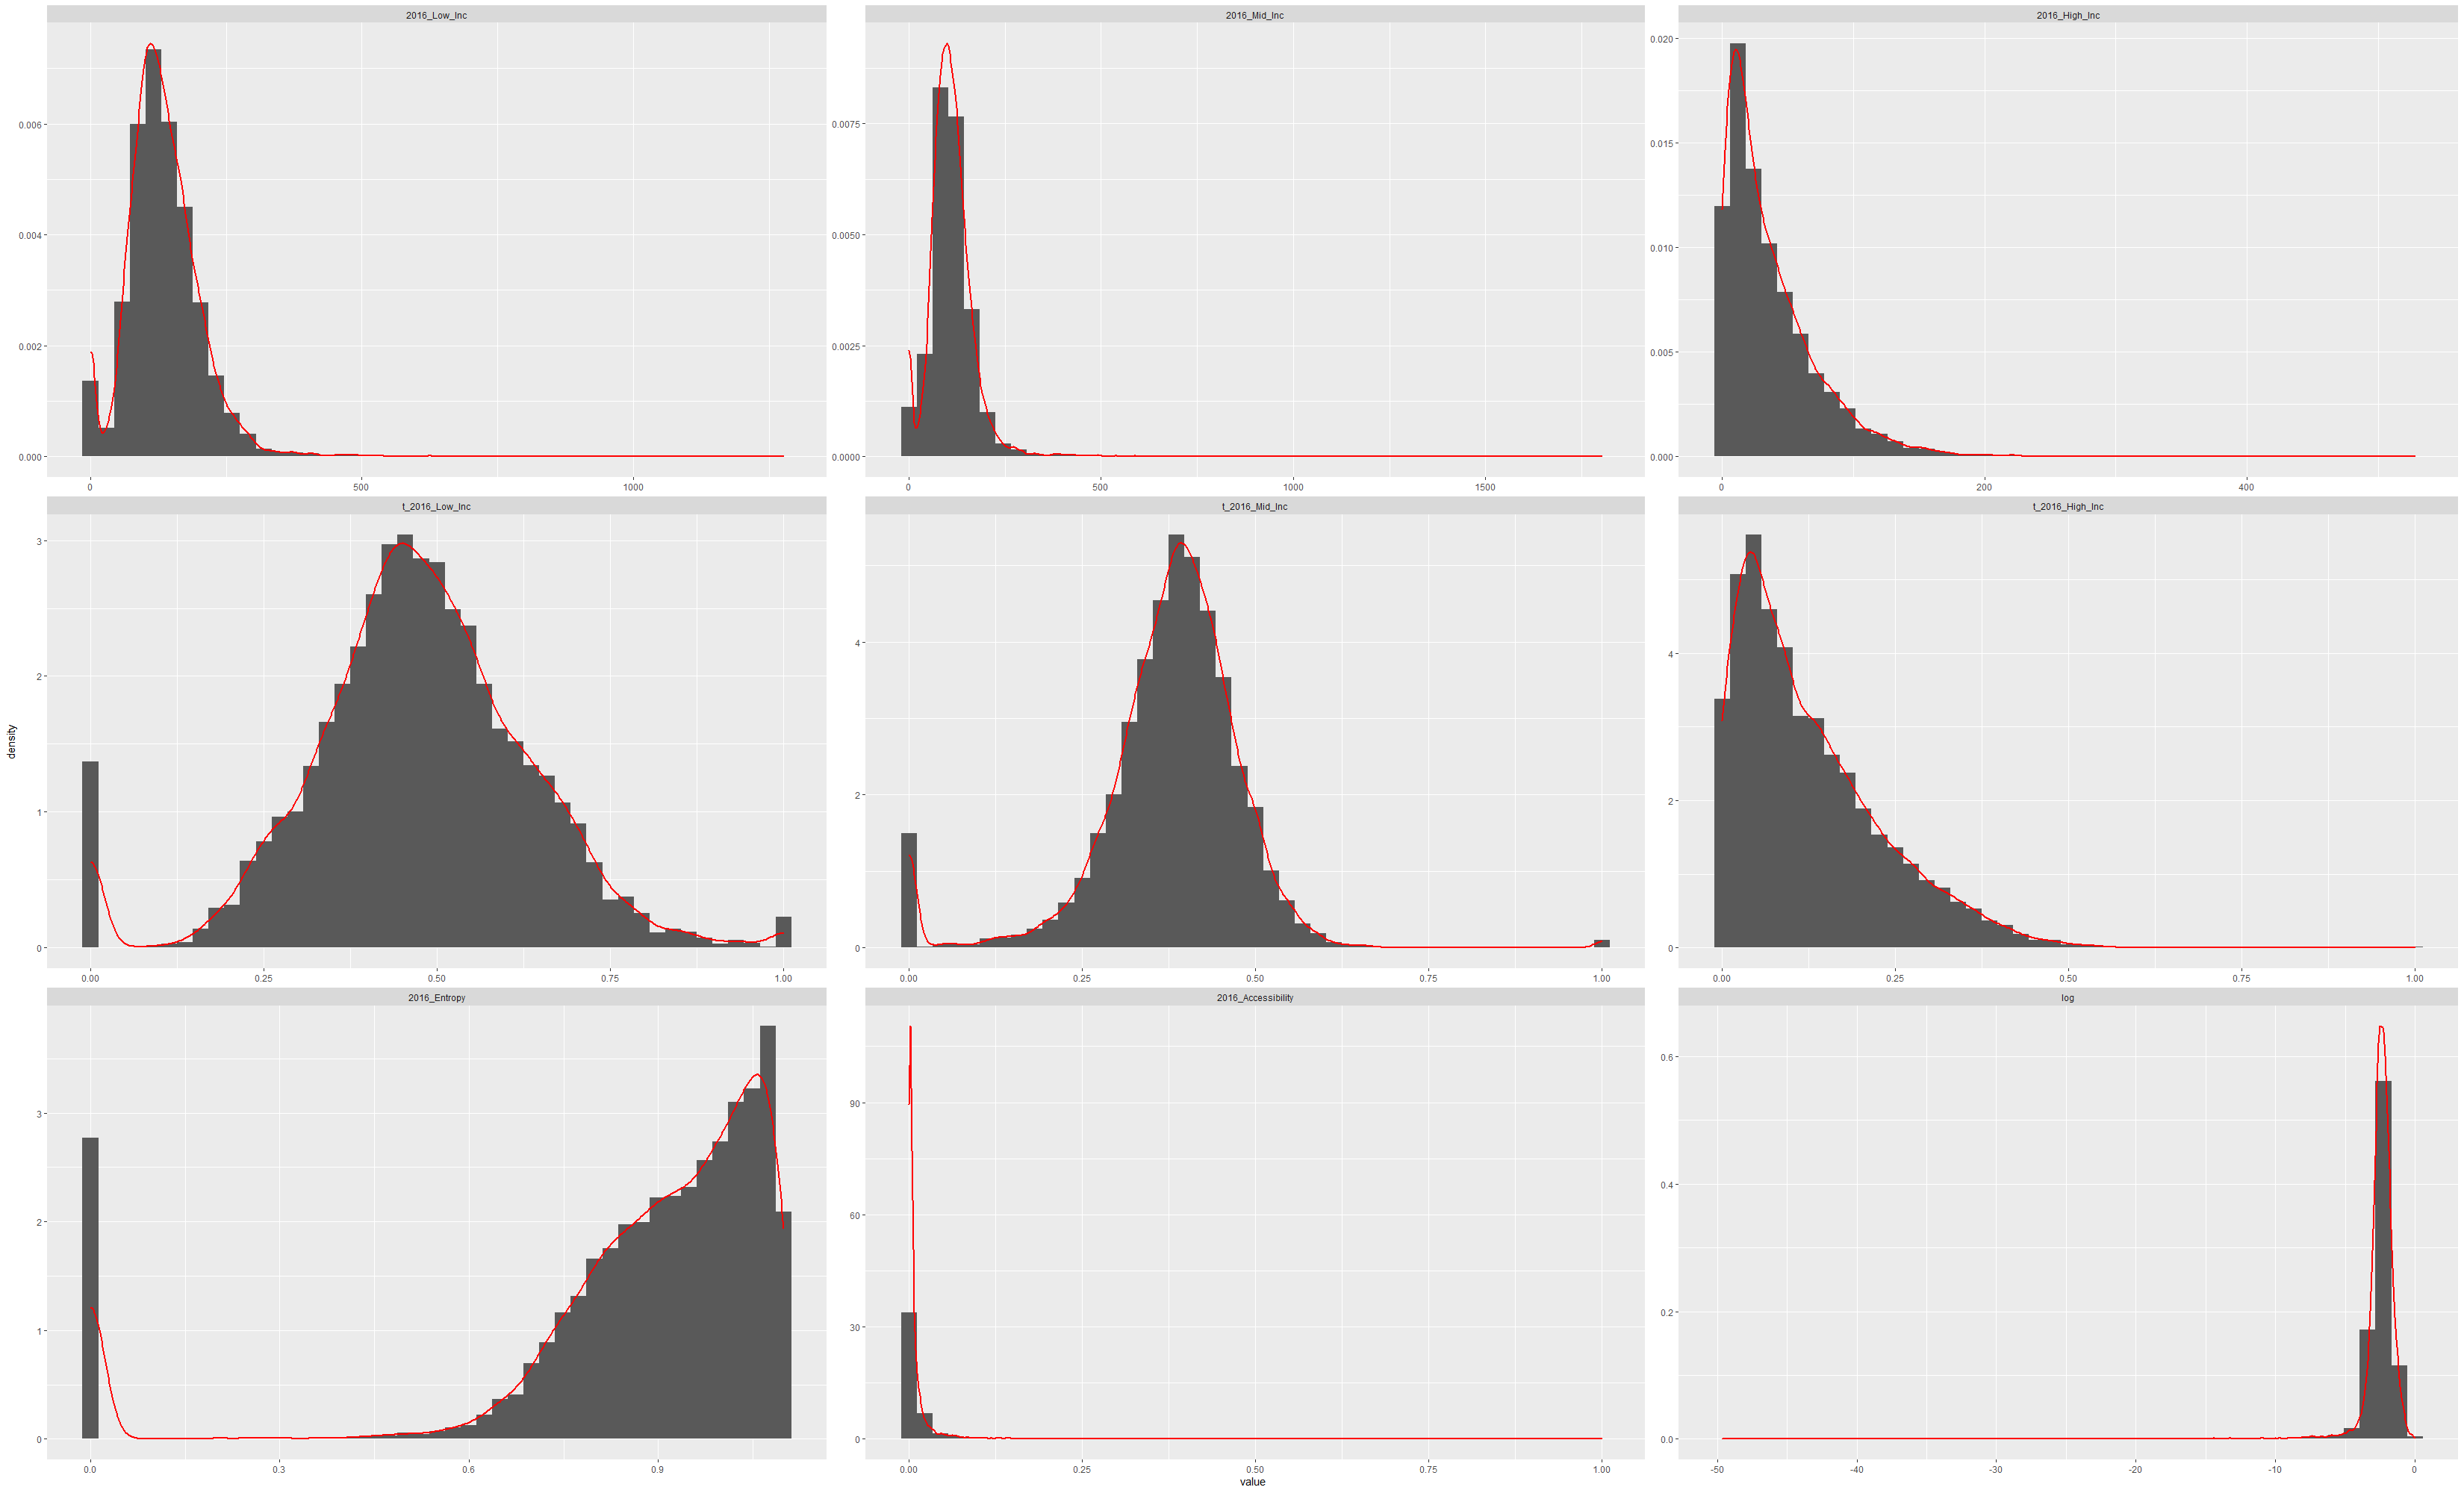
\includegraphics[width=1\textwidth]{body/figures/Rplot01.png}
    \caption{Caption}
    \label{fig:my_label}
\end{figure}

\subsection{House Price}

\begin{figure}[!ht]
    \centering
    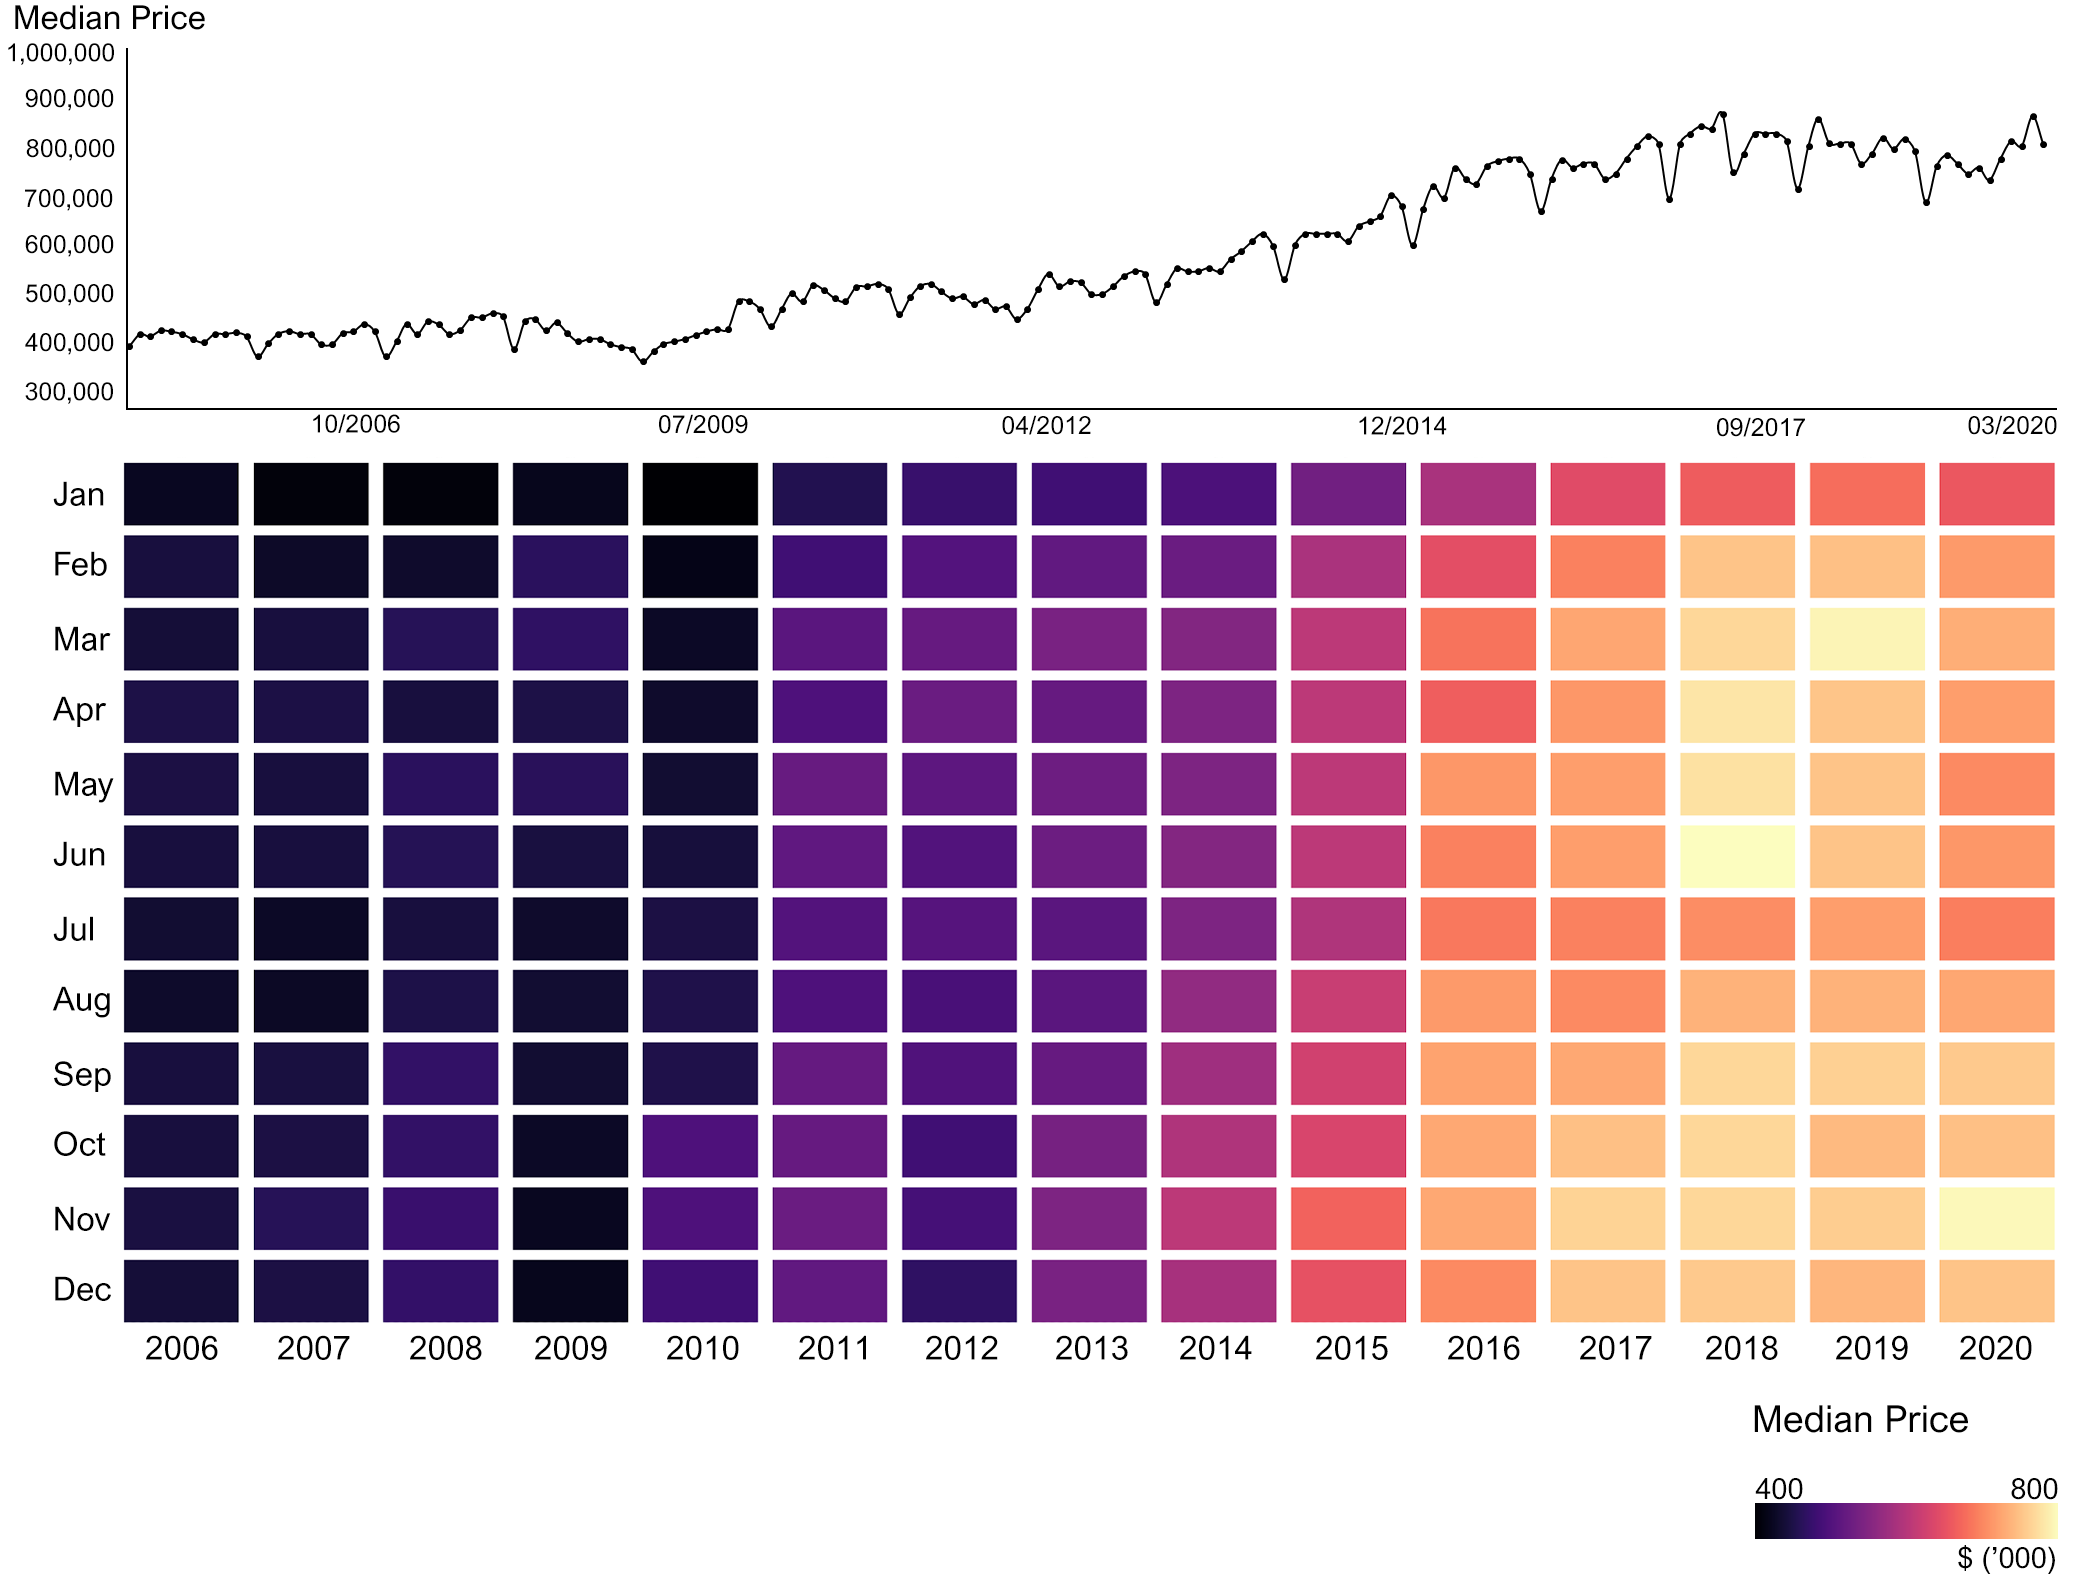
\includegraphics[width=1\textwidth]{body/figures/house_price_data.png}
    \caption{Caption}
    \label{fig:my_label}
\end{figure}

\begin{figure}[!ht]
    \centering
    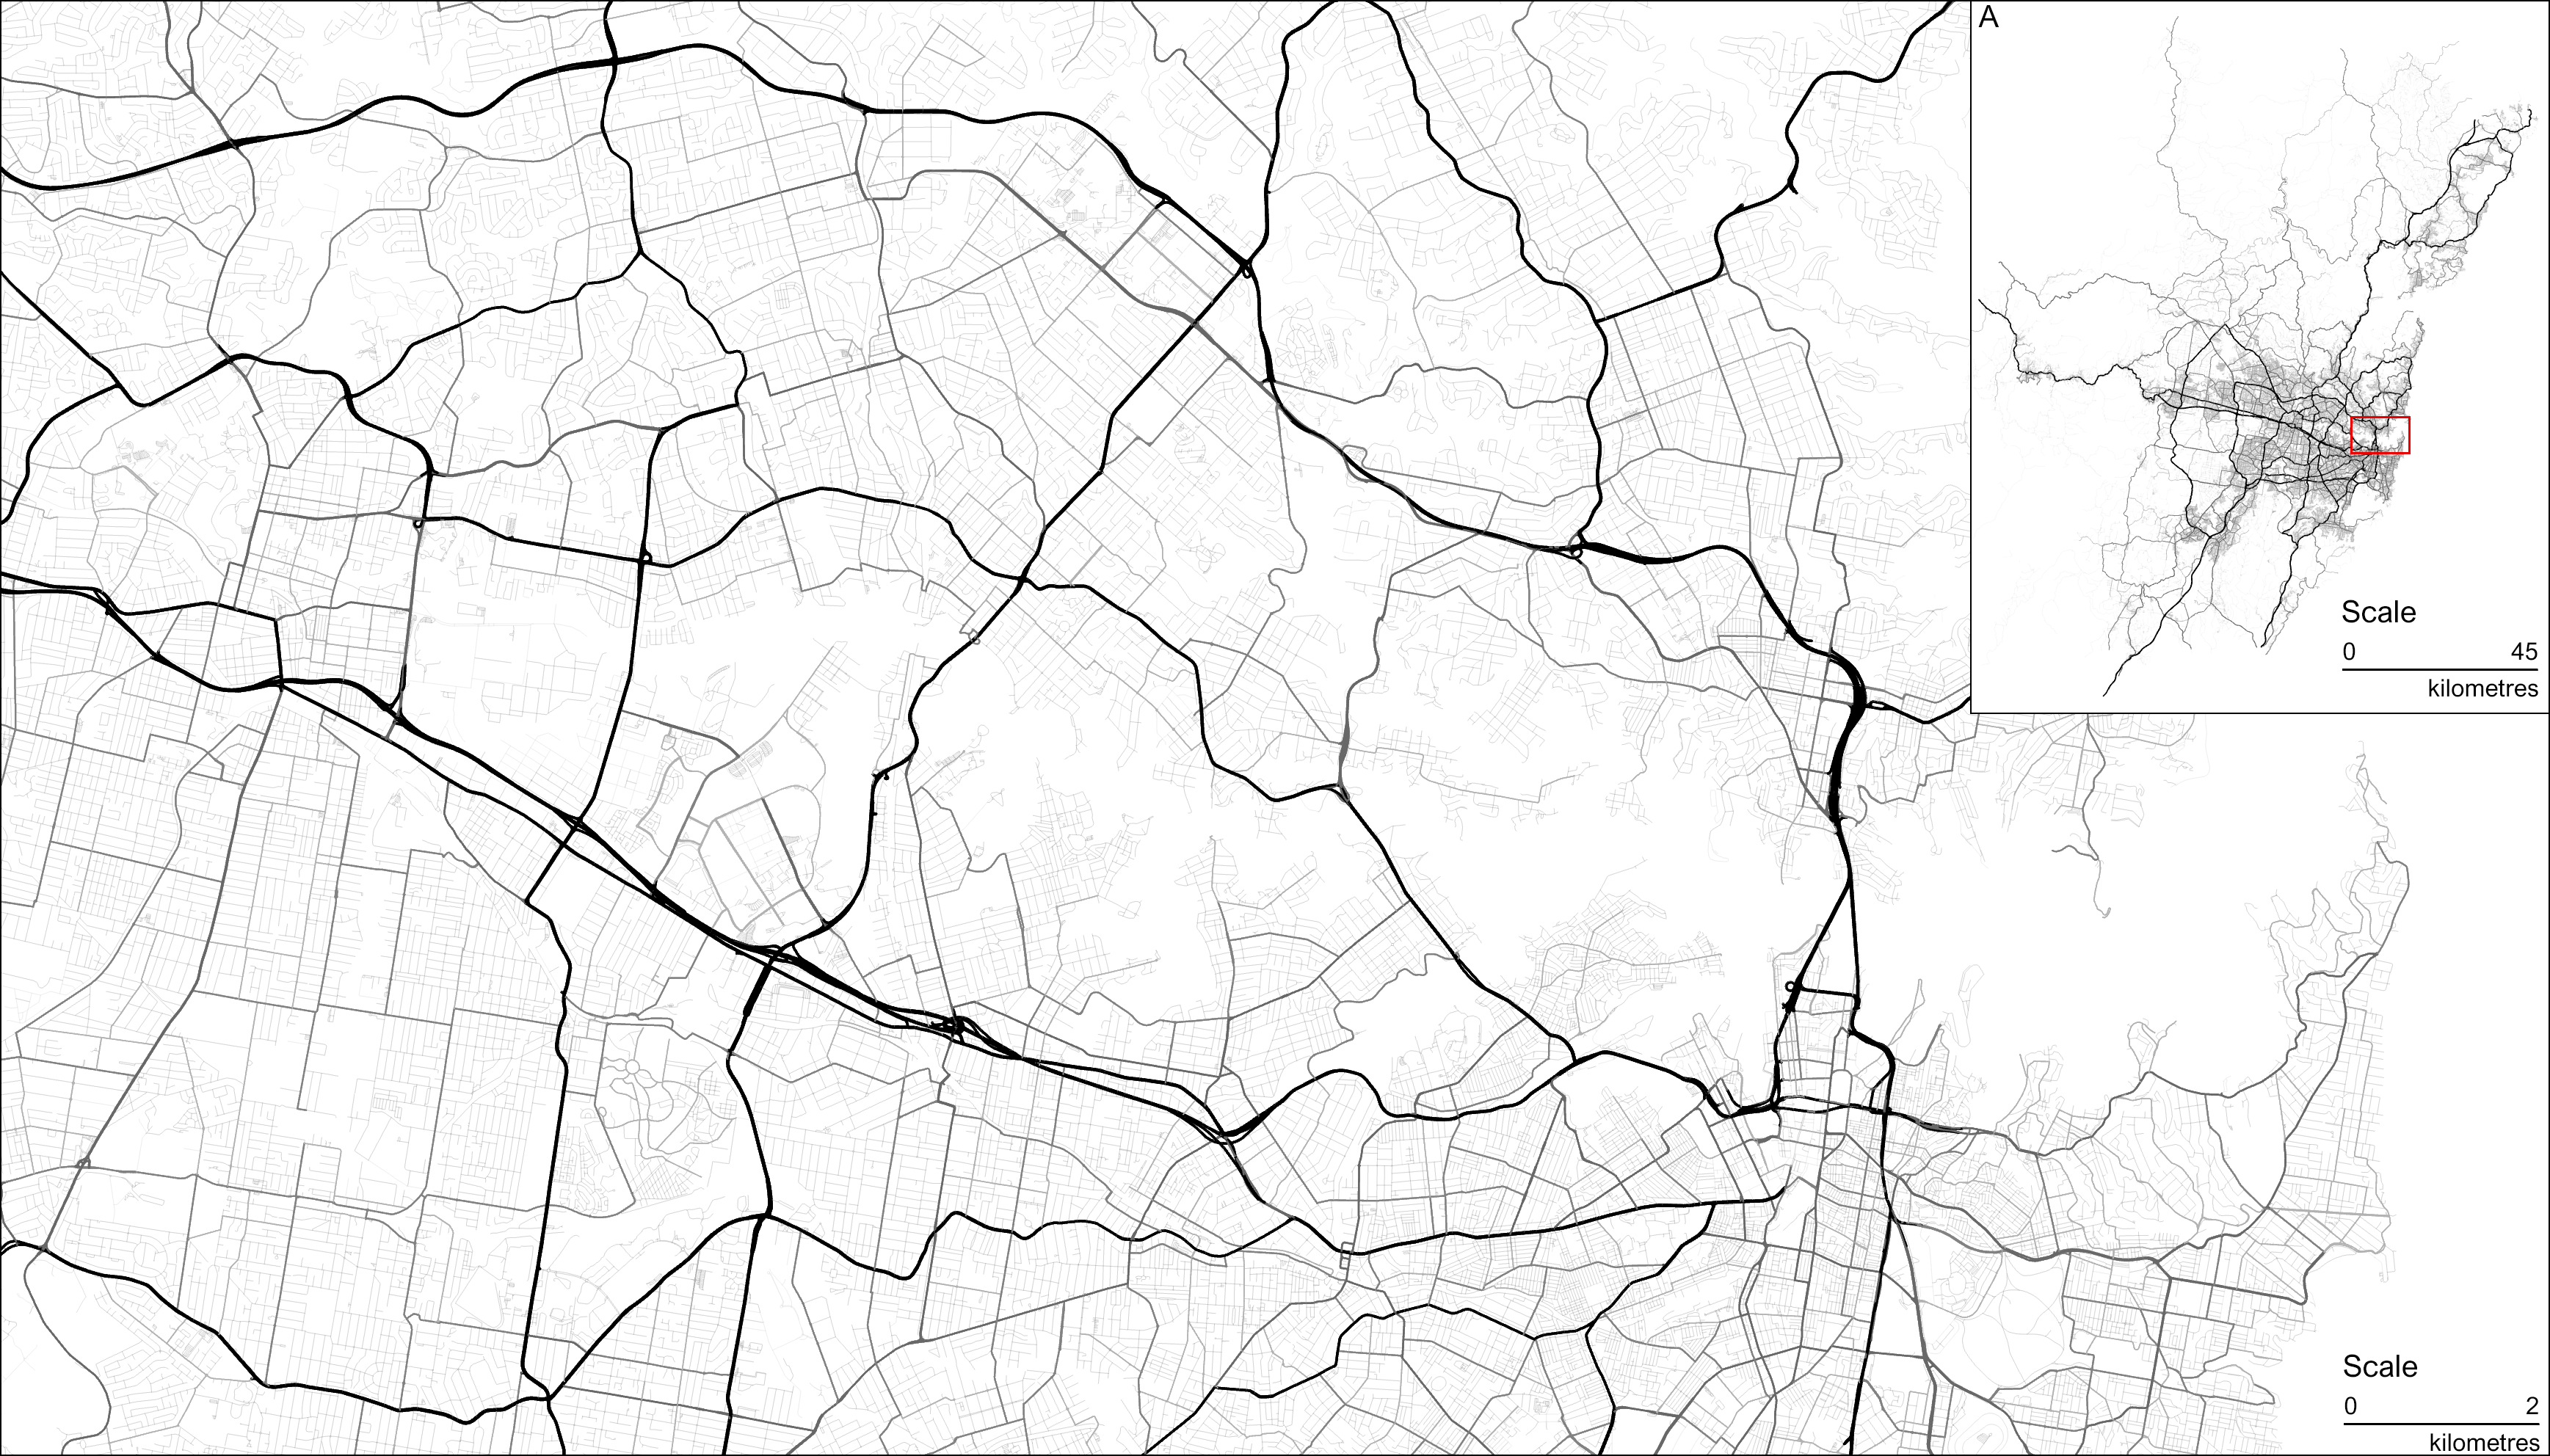
\includegraphics[width=1\textwidth]{body/figures/road.png}
    \caption{Caption}
    \label{fig:my_label}
\end{figure}


\begin{figure}[!ht]
    \centering
    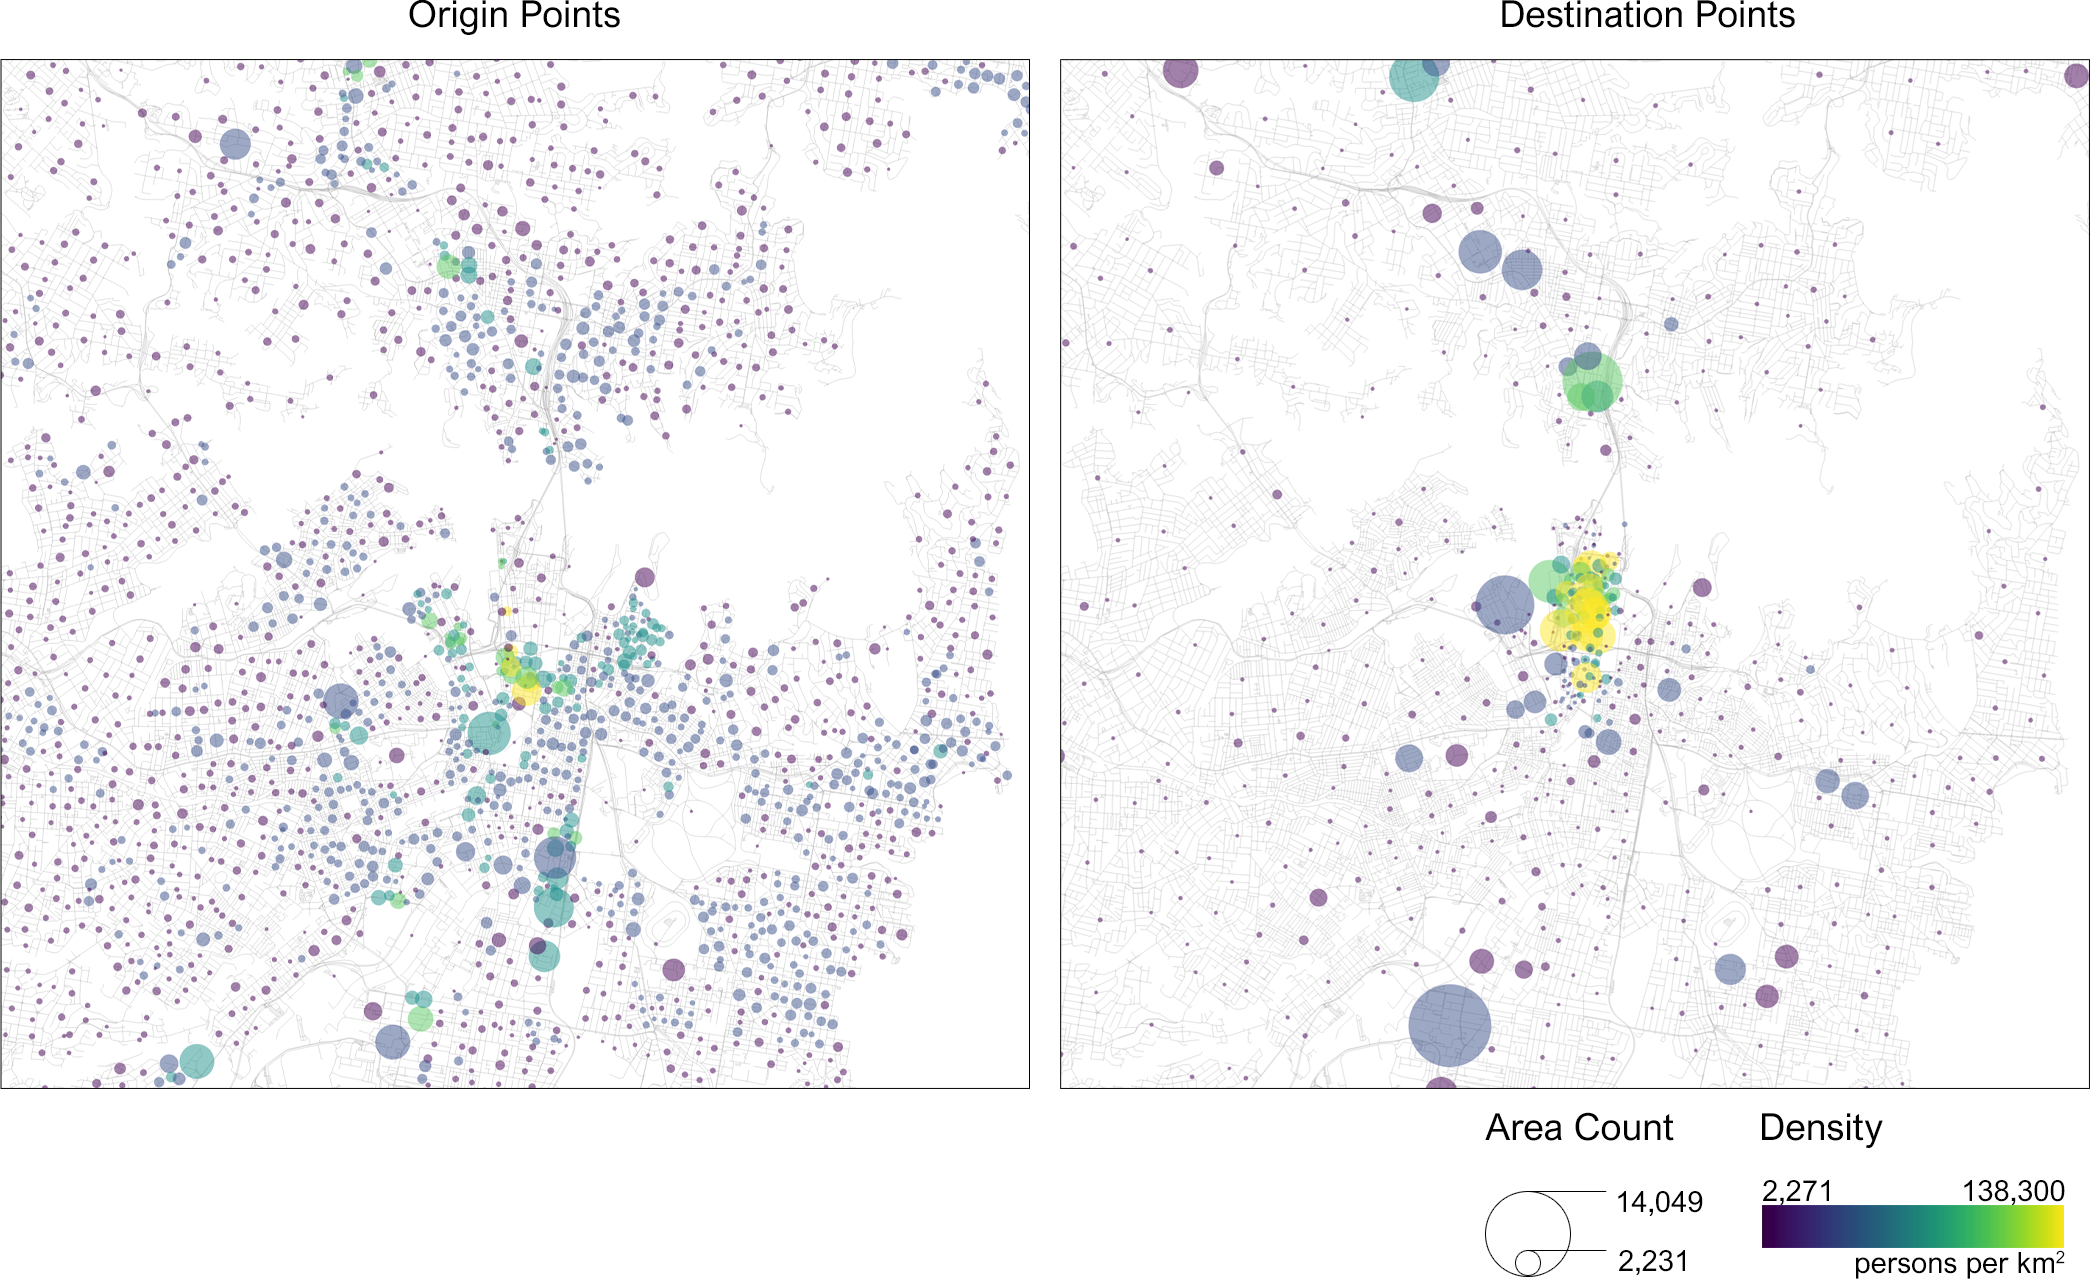
\includegraphics[width=1\textwidth]{body/figures/od_points.png}
    \caption{Caption}
    \label{fig:my_label}
\end{figure}

\begin{figure}[!ht]
    \centering
    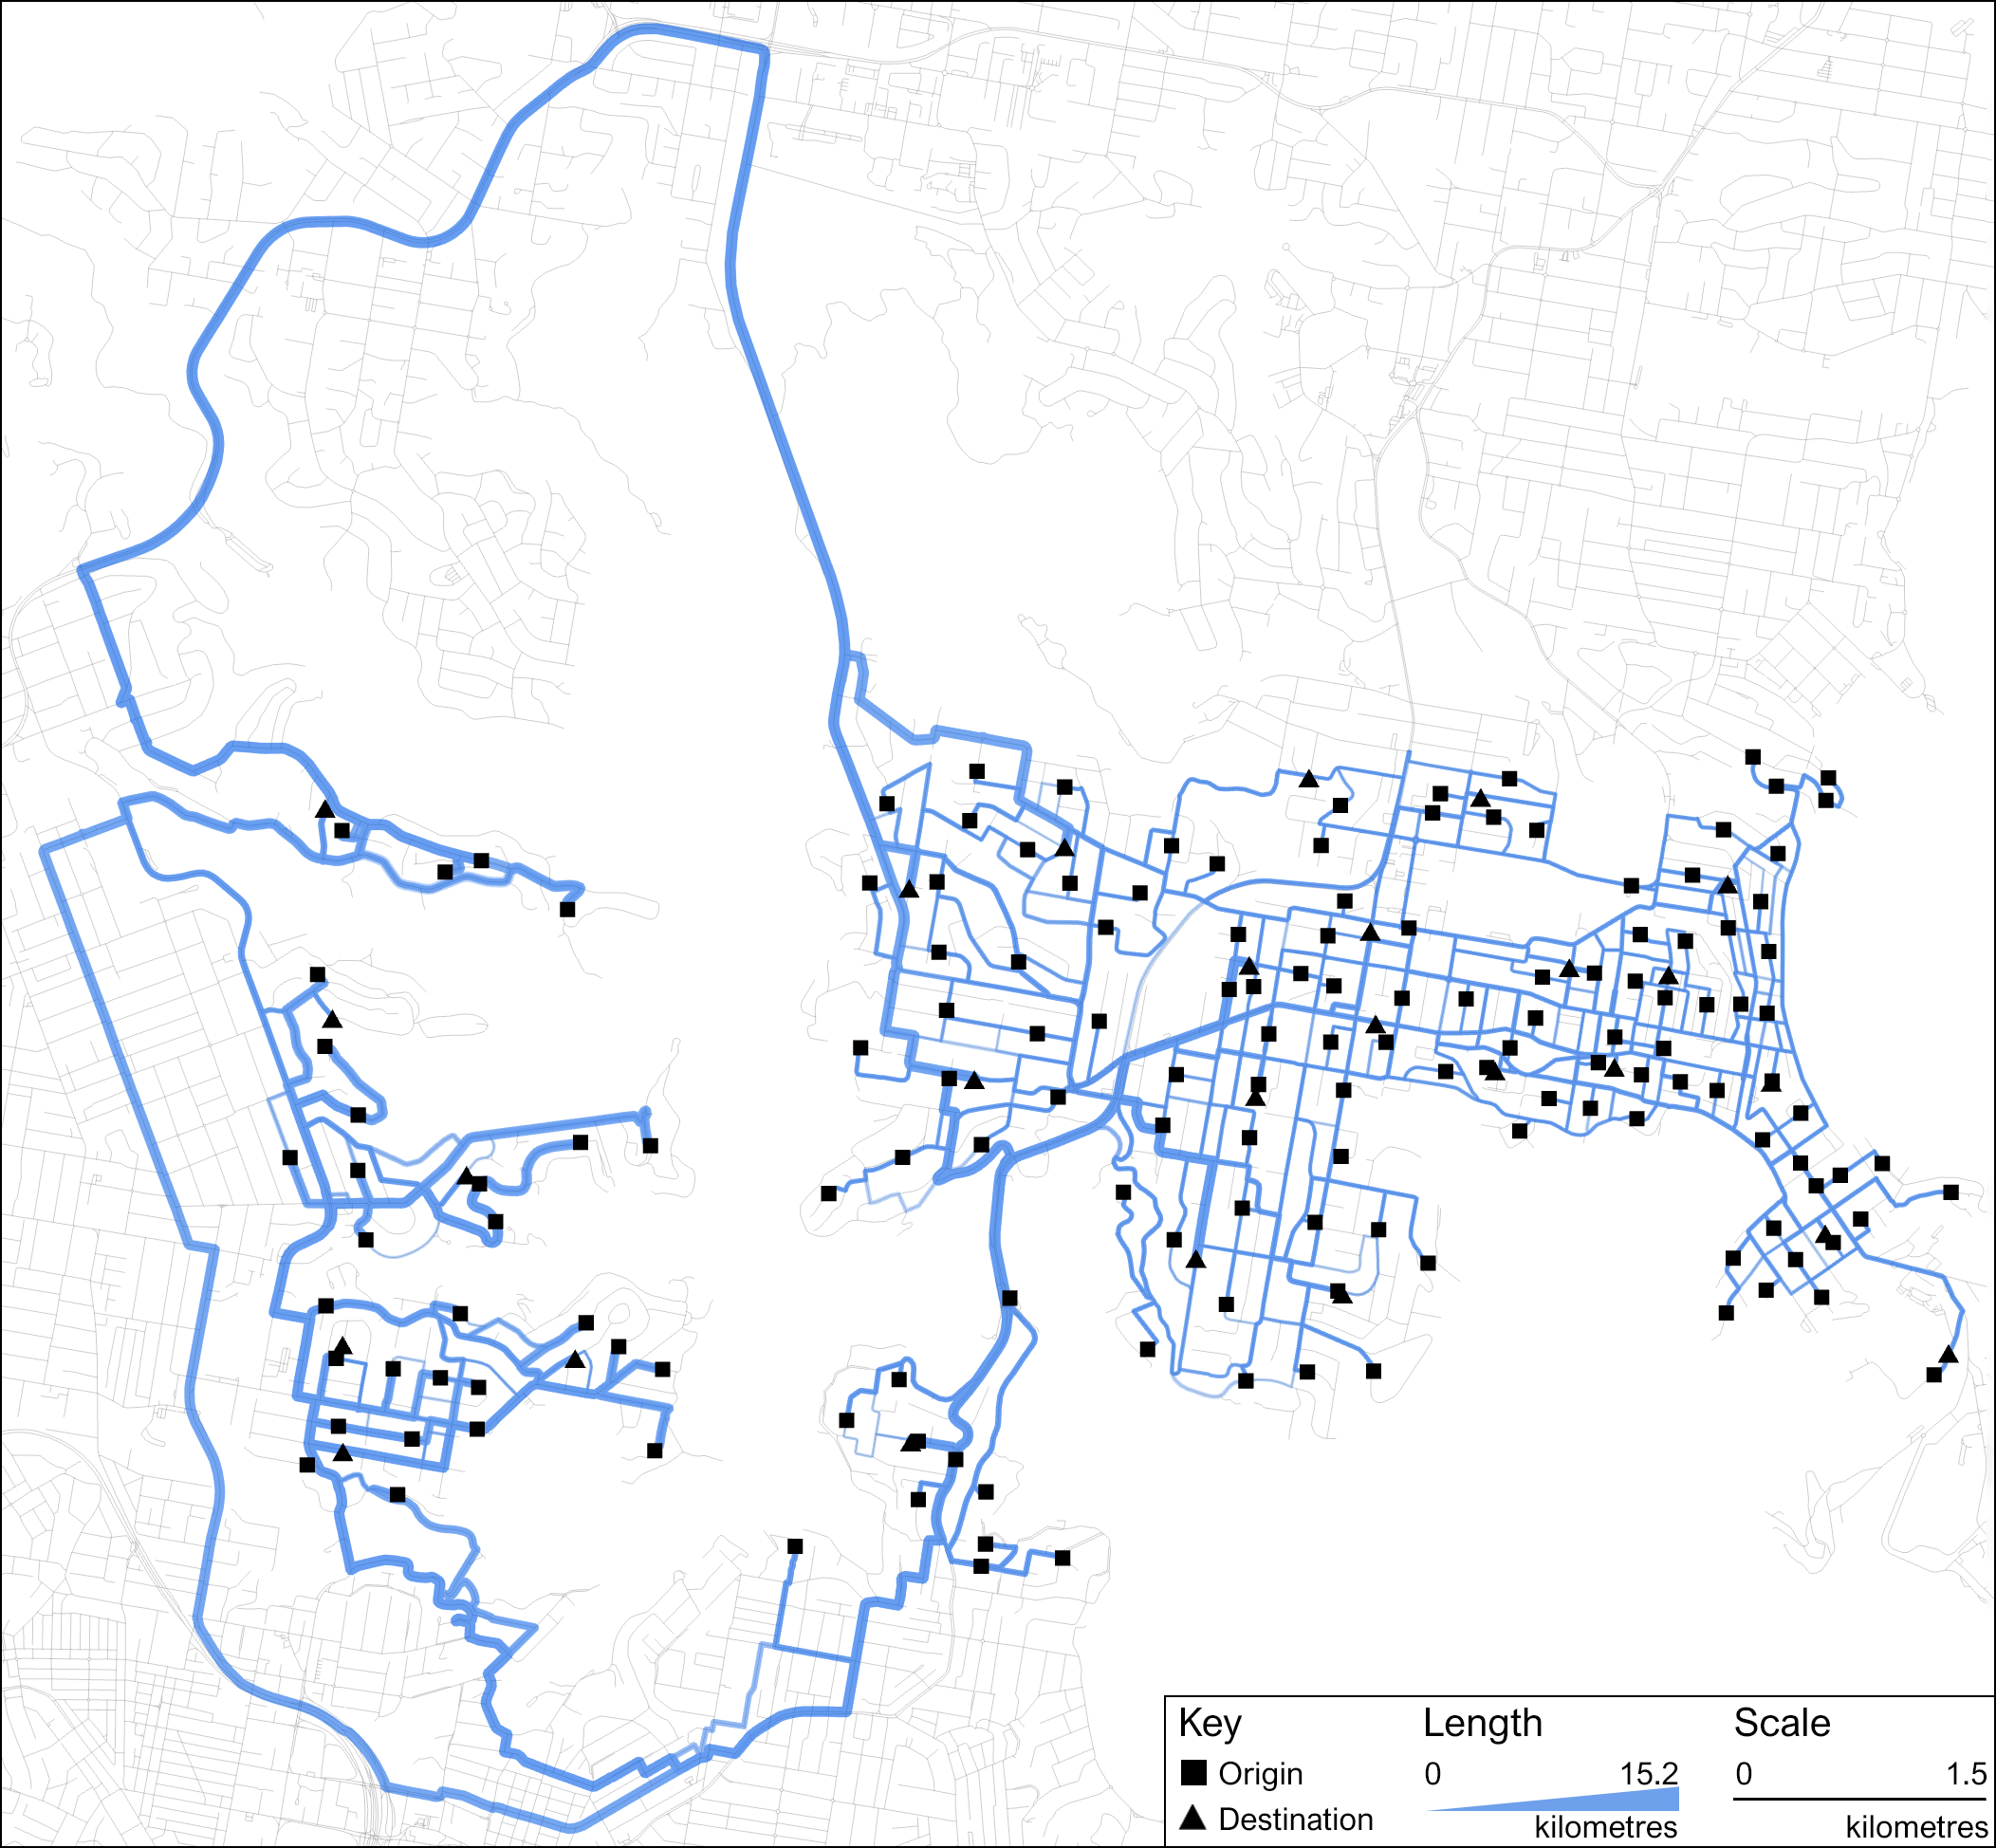
\includegraphics[width=0.85\textwidth]{body/figures/OD1.png}
    \caption{Caption}
    \label{fig:my_label}
\end{figure}


\section{Methods}

\subsection{Accessibility Indices}

\begin{equation}
T_{ij} = k\frac{V_{i}^{\mu} W_{j}^{\alpha}}{f(d_{ij})}
\end{equation}

\begin{equation}
    T = \sum_{i}\sum_{j}T_{ij}
\end{equation}

\begin{equation}
    ln T_{ij} = k + \mu ln(V_{i}) + \alpha ln(W_{j}) - \beta ln(d_{ij})
\end{equation}

\begin{equation}
    \sum_{j}T_{ij} = O_{i}
\end{equation}

\begin{equation}
    A_i = \frac{1}{\sum_{j}W^{\alpha}_{j} \cdot f({d_{ij})}}
\end{equation}

\begin{equation}
    T_{ij} = A_{i}\cdot O_{i} \cdot W_{j}^{\alpha} \cdot f(d_{ij})
\end{equation}

\begin{equation}
    \delta_{ij} = exp(\sigma_{i} + \alpha ln W_{j} - \beta ln d_{ij}) 
\end{equation}

2011: $R^{2}$ = 0.493

2016: $R^{2}$ = 0.521

\subsubsection{Model Parameterisation}

\begin{equation}
    f(d_{ij}) = exp^{-\beta \cdot d_{ij}}
\end{equation}

\begin{equation}
    f(d_{ij}) = d_{ij}^{-\beta}
\end{equation}

\subsection{Entropy}

\begin{figure}[p]
    \centering
    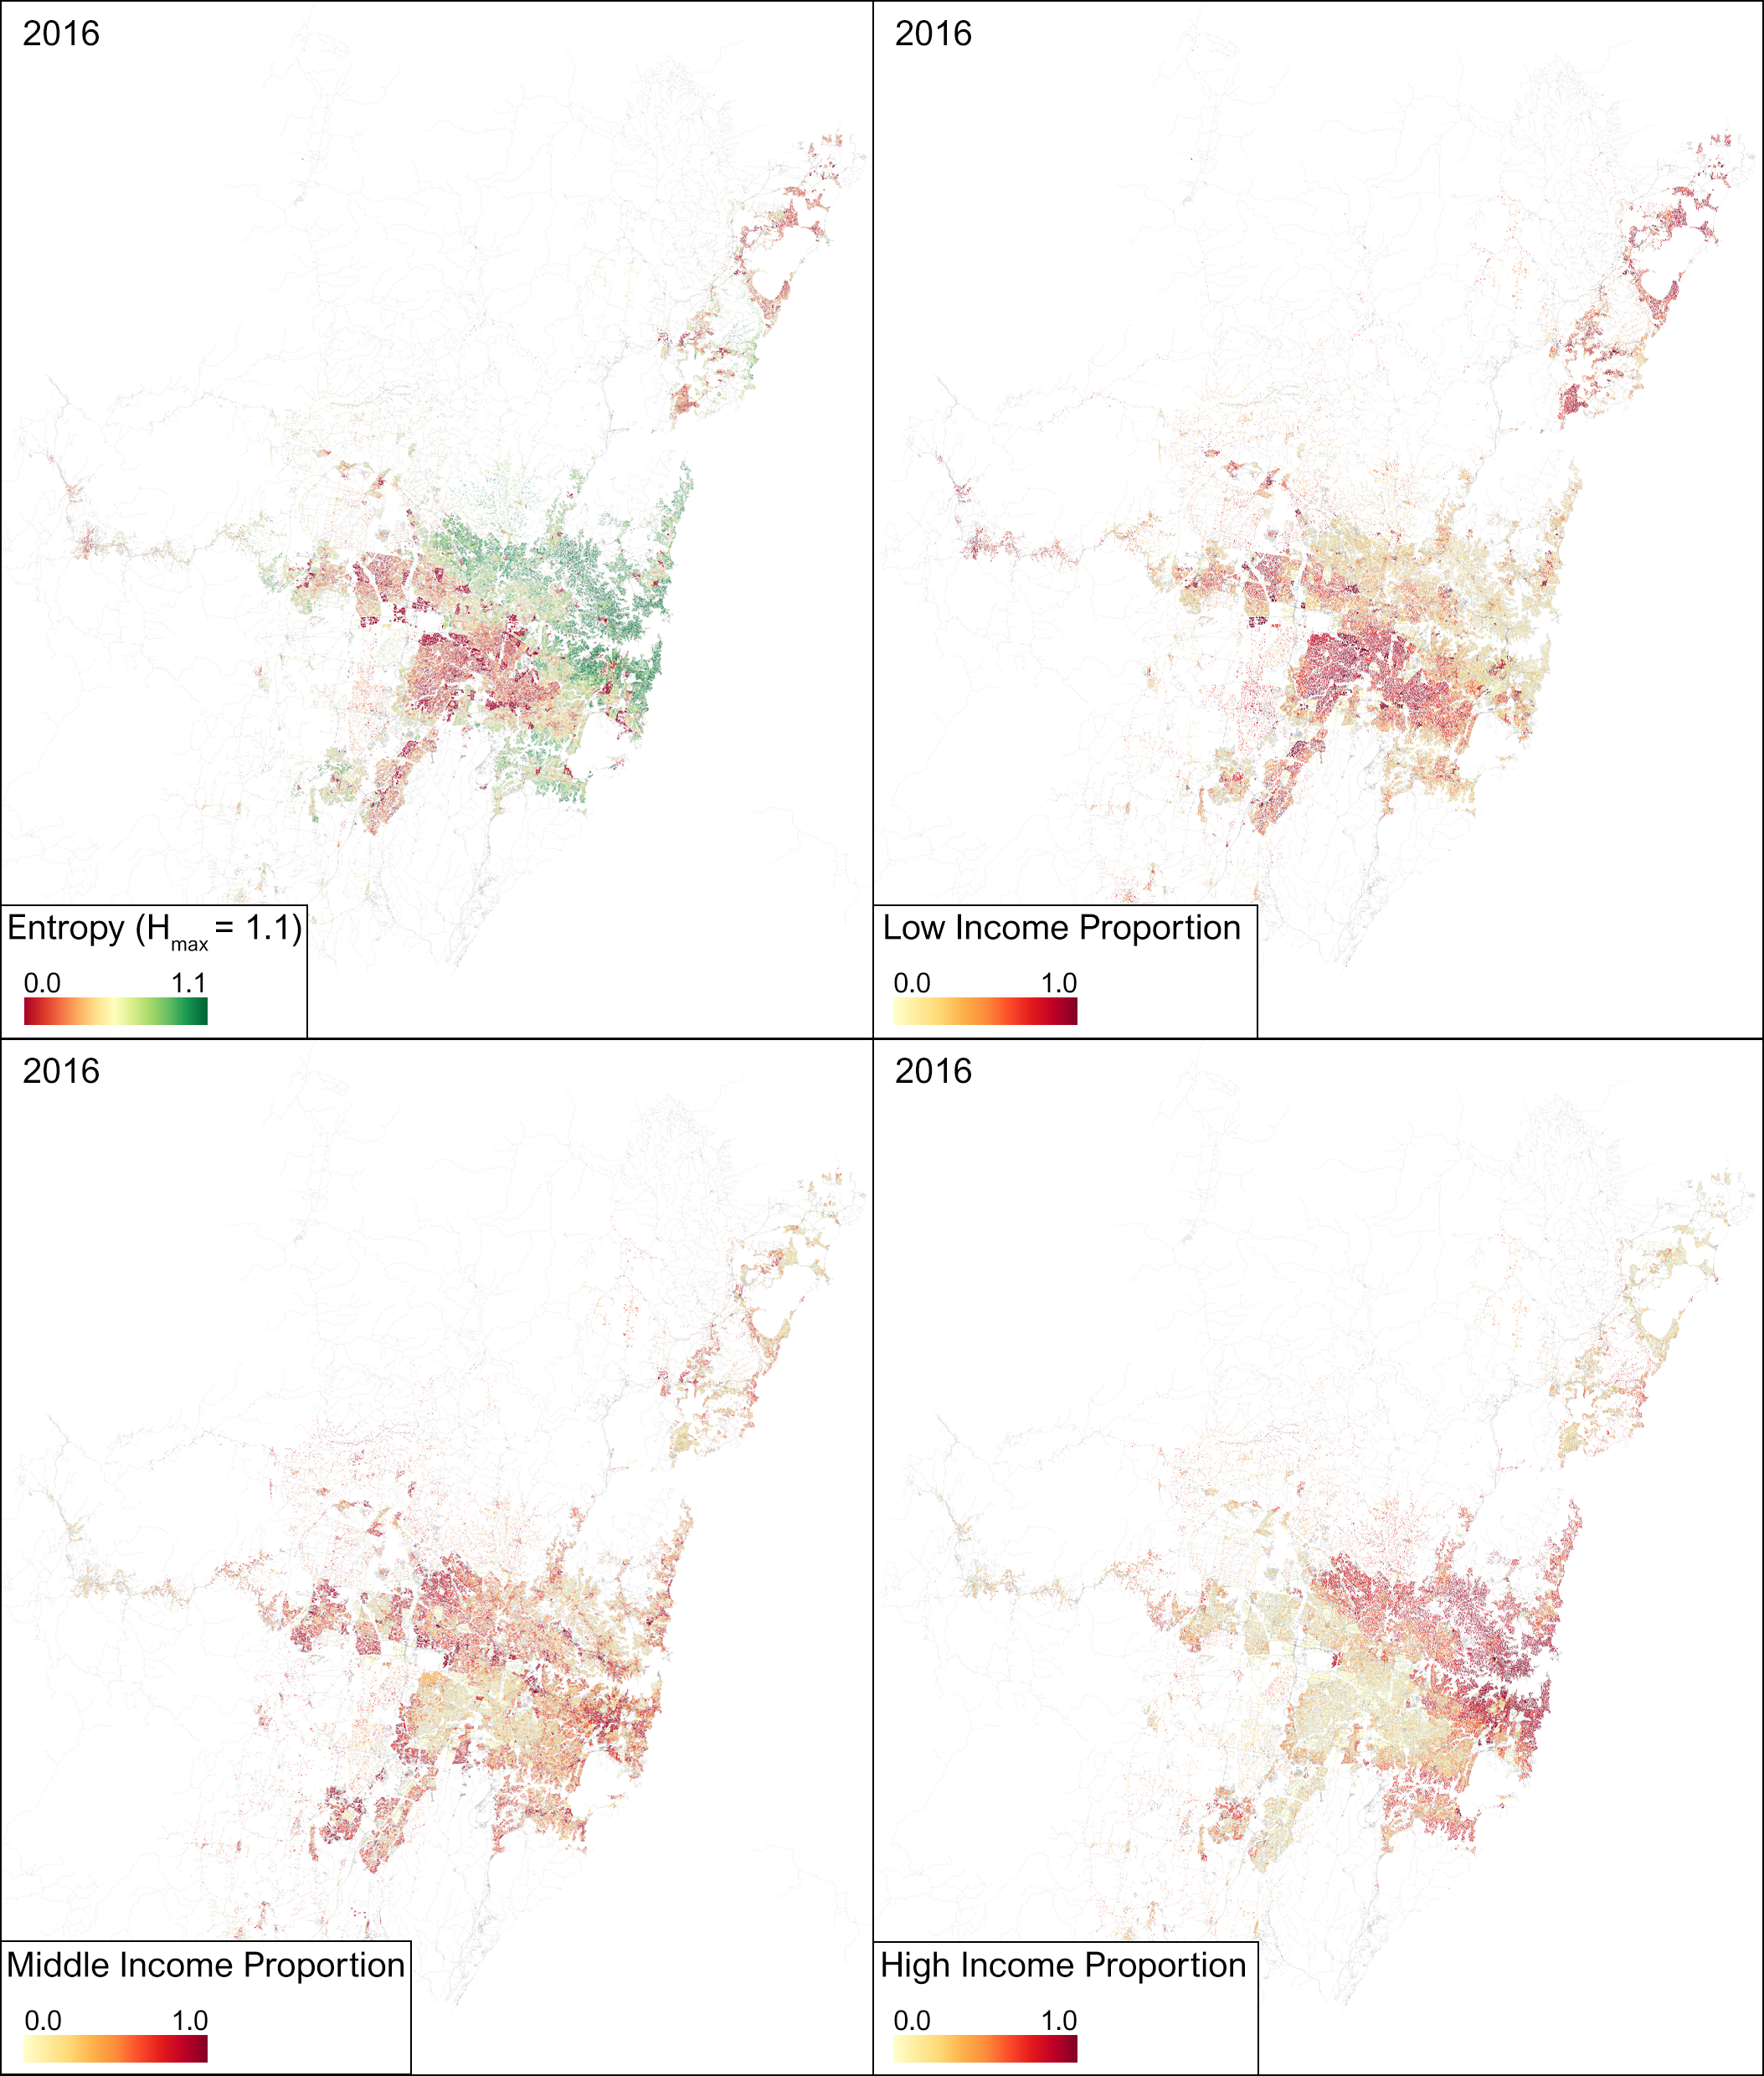
\includegraphics[width=1\textwidth]{body/figures/Income_Proportion_16.png}
    \caption{Caption}
    \label{fig:my_label}
\end{figure}

\begin{equation}
    H_{i} = - \sum^{k}_{j=1}P_{ij} \cdot ln(P_{ij})
\end{equation}

\begin{equation}
    P_{ij} = \frac{P_{ij}}{\sum_{j=1}^{k}P_{ij}}
\end{equation}

\begin{equation}
    H_{max} = ln(k)
\end{equation}

\subsection{Exposure Index}

\begin{equation}
    P = \sum^{n}_{i=1}(\frac{P_{1i}}{P_{i}})(\frac{P_{2i}}{T_i})
\end{equation}

\begin{figure}[H]
    \centering
    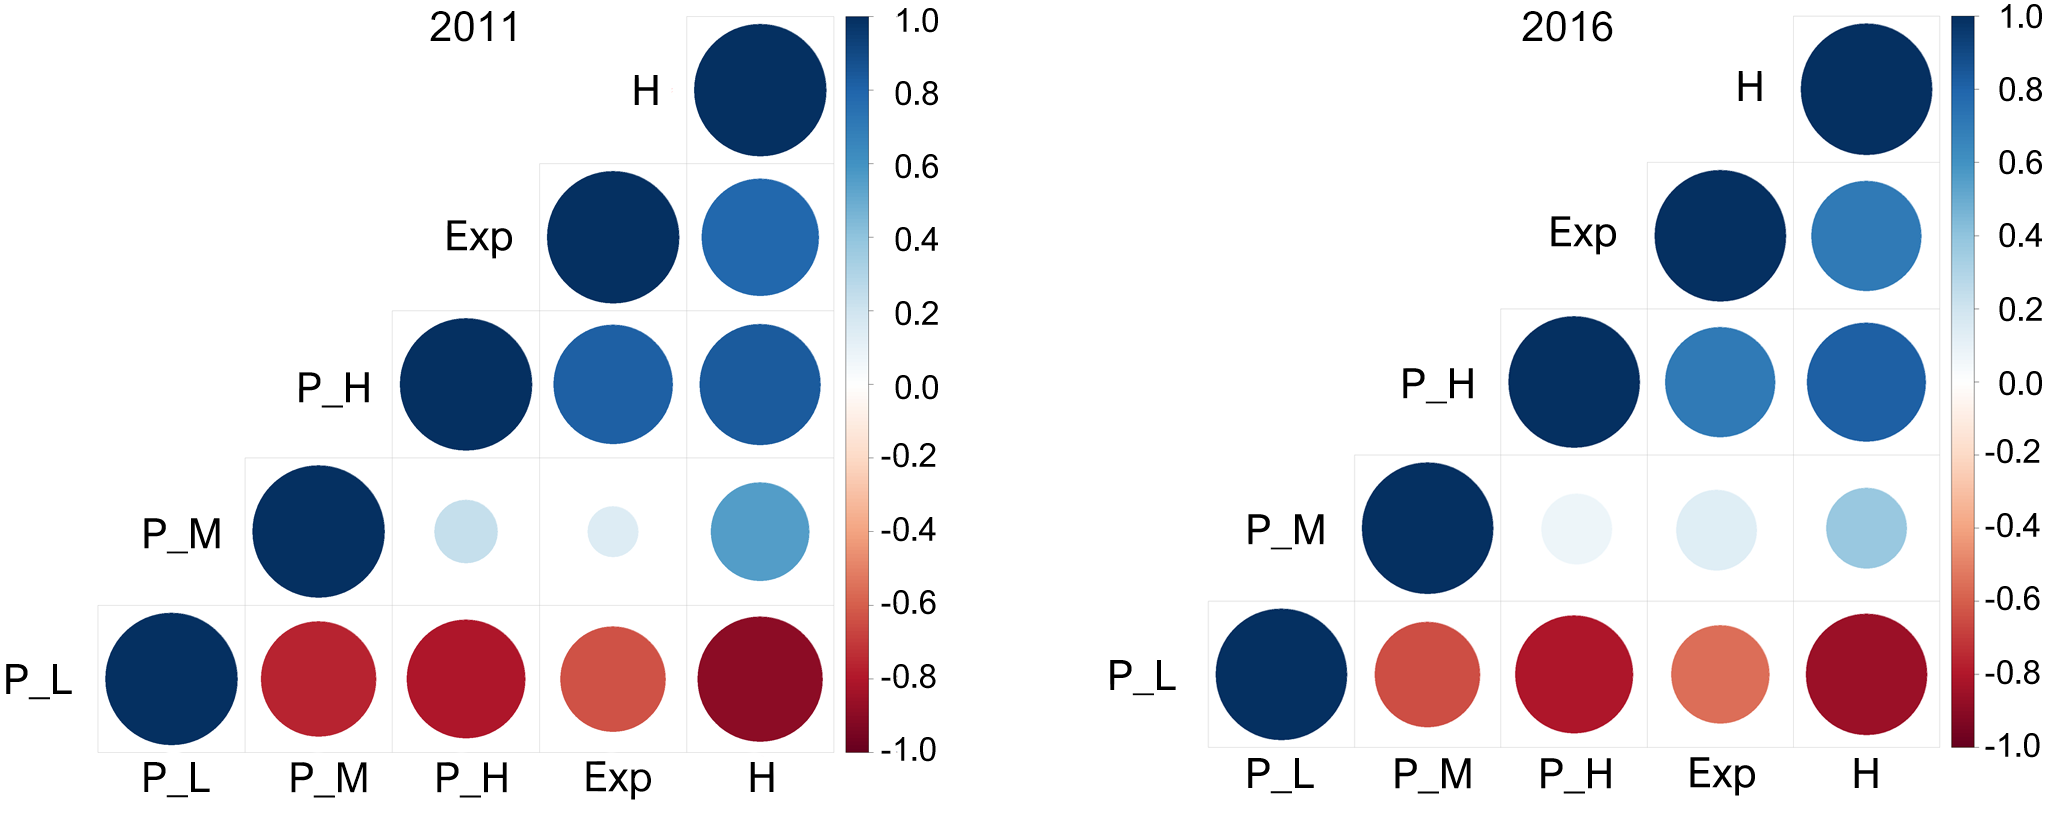
\includegraphics[width=1\textwidth]{body/figures/Entropy_CorrPlot.png}
    \caption{Correlogram of Census tract income classes against the Low-High Income Exposure Index, and the standardised entropy values. N.b. \textbf{P\_L}: Census tract proportion of low-income groups; Census tract proportion of middle-income groups; \textbf{P\_H}: Census tract proportion of high-income groups; \textbf{Exp}: Low-High Exposure Index; \textbf{H}: Entropy Index.}
    \label{fig:Correlogram}
\end{figure}

\subsection{Geographically Weighted Regression}
 We take into account spatial variance of house location on their price. The GWR uses coordinates of each sample point, 

Fotheringham et al (1998) first introduced the geographically weighted regression (GWR) to account for spatially varying parameters

The regression is based on hyperlocal regression as observed at each location points - this disaggregation an entirely different set of coefficients to be predicted than a non-spatial OLS model. 

OLS Model

\begin{equation}
    y = \beta_{0} + \beta_{1}x_{1} + \beta_{2}x_{2} + ... + \varepsilon
\end{equation}

the slope and intercept parameters are global, in the sense that they apply to all observations. 

GWR the dependent variable at location $i$ is modelled as: 

\begin{equation}
    y_{i} = \beta_{i0} + \sum^{N}_{j=1}\beta_{ij}x_{ij} + \varepsilon_{i}
\end{equation}

the coefficients , $\beta$, varies spatially, and are determined with this spatial variation through their coordinate locations. 
The model resembles a linear regression, with $N$ independent variables 

\begin{equation}
    w_{ij} =\left (1 - \frac{d_{ij}^2}{b^{2}}  \right )^{2},\; if \; d_{ij} < r, \; 0 \; otherwise
\end{equation}

MGWR

\begin{equation}
y_{i} = \beta_{bw0} + \sum_{k} \alpha_{bwk} x_{ik} + \varepsilon_{i}
\end{equation}

\section{Results}
\renewcommand{\baselinestretch}{0.8}
\begin{table}[!ht]
  \centering \small
  \caption{Add caption}
    \begin{tabular}{llllll}
    \multicolumn{6}{l}{\textbf{Residuals}} \\
    \midrule
    & \multicolumn{1}{c}{\textbf{Min}} & \multicolumn{1}{c}{\textbf{1Q}} & \multicolumn{1}{c}{\textbf{Median}} & \multicolumn{1}{c}{\textbf{3Q}} & \multicolumn{1}{c}{\textbf{Max}}   \\
    &\multicolumn{1}{c}{-1.3009} & \multicolumn{1}{c}{-0.06182} & \multicolumn{1}{c}{-0.00785} & \multicolumn{1}{c}{0.04952} & \multicolumn{1}{c}{1.08721}   \\
          &       &       &       &       &  \\
    \textbf{Coefficients:} &       &       &       &       &  \\
    \midrule
          & \textbf{Estimate} & \textbf{Standard Error} & \textbf{value} & \textbf{Pr($>$ $|$ t $|$)} &  \\
    (Intercept) & \multicolumn{1}{r}{5.81E+00} & \multicolumn{1}{r}{3.62E-02} & \multicolumn{1}{r}{160.778} & $<$2.0E-16 & *** \\
    Bedrooms & \multicolumn{1}{r}{3.87E-02} & \multicolumn{1}{r}{1.19E-03} & \multicolumn{1}{r}{32.497} & $<$2.0E-16 & *** \\
    Baths & \multicolumn{1}{r}{4.20E-02} & \multicolumn{1}{r}{1.48E-03} & \multicolumn{1}{r}{28.311} & $<$2.0E-16 & *** \\
    Parking & \multicolumn{1}{r}{1.86E-02} & \multicolumn{1}{r}{9.12E-04} & \multicolumn{1}{r}{20.37} & $<$2.0E-16 & *** \\
    Distance to Sydney City & \multicolumn{1}{r}{-5.22E-06} & \multicolumn{1}{r}{9.03E-08} & \multicolumn{1}{r}{-57.874} & $<$2.0E-16 & *** \\
    Distance to Secondary Cities & \multicolumn{1}{r}{1.87E-07} & \multicolumn{1}{r}{9.74E-08} & \multicolumn{1}{r}{1.914} & 0.056 & . \\
    Distance to Beach & \multicolumn{1}{r}{-1.41E-06} & \multicolumn{1}{r}{1.27E-07} & \multicolumn{1}{r}{-11.051} & $<$2.0E-16 & *** \\
    Distance to Shopping Centres & \multicolumn{1}{r}{8.73E-06} & \multicolumn{1}{r}{3.29E-07} & \multicolumn{1}{r}{26.578} & $<$2.0E-16 & *** \\
    Unemployment Rate & \multicolumn{1}{r}{-4.08E-03} & \multicolumn{1}{r}{6.87E-04} & \multicolumn{1}{r}{-5.942} & 0.000 & *** \\
    Median Personal Income & \multicolumn{1}{r}{-3.36E-05} & \multicolumn{1}{r}{1.18E-05} & \multicolumn{1}{r}{-2.856} & 0.004 & ** \\
    Crime Rate & \multicolumn{1}{r}{-5.85E-02} & \multicolumn{1}{r}{1.04E-02} & \multicolumn{1}{r}{-5.623} & 0.000 & *** \\
    Low Income (\%) & \multicolumn{1}{r}{-1.90E-02} & \multicolumn{1}{r}{3.63E-02} & \multicolumn{1}{r}{-0.522} & 0.601 &  \\
    Middle Income (\%) & \multicolumn{1}{r}{-1.12E-01} & \multicolumn{1}{r}{3.65E-02} & \multicolumn{1}{r}{-3.07} & 0.002 & ** \\
    High Income (\%) & \multicolumn{1}{r}{1.15E+00} & \multicolumn{1}{r}{4.04E-02} & \multicolumn{1}{r}{28.388} & $<$2.0E-16 & *** \\
    Accessibility Score & \multicolumn{1}{r}{3.78E-05} & \multicolumn{1}{r}{3.06E-06} & \multicolumn{1}{r}{12.341} & $<$2.0E-16 & *** \\
    \midrule
    \multicolumn{6}{l}{Significance Codes:} \\
    \multicolumn{6}{c}{\textit{0 ‘***’ 0.001 ‘**’ 0.01 ‘*’ 0.05 ‘.’ 0.1 ‘ ’ 1}} \\
    \multicolumn{6}{l}{\textit{Number of data points: 14,868}} \\
    \multicolumn{6}{l}{\textit{Residual standard error: 0.1046 on 14853 degrees of freedom}} \\
    \multicolumn{6}{l}{\textit{Multiple R-squared:  0.8173, 	Adjusted R-squared:  0.8171 }} \\
    \multicolumn{6}{l}{\textit{F-statistic:  4745 on 14 and 14853 DF,  p-value: $<$ 2.2e-16}} \\
    \multicolumn{6}{l}{Diagnostic Information:} \\
    \multicolumn{6}{l}{\textit{Residual sum of squares: 162.5161}} \\
    \multicolumn{6}{l}{\textit{$\hat{\sigma}$: 0.1045565}} \\
    \multicolumn{6}{l}{\textit{AIC:  -24,921.15}} \\
    \multicolumn{6}{l}{\textit{AICc:  -24,921.11}} \\
    \end{tabular}%
    \caption{Add caption}
  \label{tab:addlabel}%
\end{table}%


\renewcommand{\baselinestretch}{0.8}
\begin{table}[htbp]
  \centering \small
    \begin{tabular}{llllll}
    \multicolumn{6}{l}{\textbf{GWR coefficient estimates:}} \\
    \midrule
          & \multicolumn{1}{r}{\textbf{Min.}} & \multicolumn{1}{r}{\textbf{1st}} & \multicolumn{1}{r}{\textbf{Median}} & \multicolumn{1}{r}{\textbf{3Q}} & \multicolumn{1}{r}{\textbf{Max.}} \\
    (Intercept) & \multicolumn{1}{r}{2.7E+00} & \multicolumn{1}{r}{5.8E+00} & \multicolumn{1}{r}{5.9E+00} & \multicolumn{1}{r}{6.1E+00} & \multicolumn{1}{r}{1.3E+01} \\
    Bedrooms & \multicolumn{1}{r}{3.2E-02} & \multicolumn{1}{r}{3.9E-02} & \multicolumn{1}{r}{4.1E-02} & \multicolumn{1}{r}{4.7E-02} & \multicolumn{1}{r}{5.8E-02} \\
    Baths & \multicolumn{1}{r}{1.1E-02} & \multicolumn{1}{r}{2.6E-02} & \multicolumn{1}{r}{3.3E-02} & \multicolumn{1}{r}{4.6E-02} & \multicolumn{1}{r}{6.2E-02} \\
    Parking & \multicolumn{1}{r}{1.0E-02} & \multicolumn{1}{r}{1.4E-02} & \multicolumn{1}{r}{1.9E-02} & \multicolumn{1}{r}{2.2E-02} & \multicolumn{1}{r}{3.5E-02} \\
    Distance to Sydney City & \multicolumn{1}{r}{-1.5E-05} & \multicolumn{1}{r}{-1.1E-05} & \multicolumn{1}{r}{-8.0E-06} & \multicolumn{1}{r}{-4.1E-06} & \multicolumn{1}{r}{0.0E+00} \\
    Distance to Secondary Cities & \multicolumn{1}{r}{-4.6E-06} & \multicolumn{1}{r}{-8.6E-07} & \multicolumn{1}{r}{6.3E-07} & \multicolumn{1}{r}{2.0E-06} & \multicolumn{1}{r}{0.0E+00} \\
    Distance to Beach & \multicolumn{1}{r}{-1.1E-05} & \multicolumn{1}{r}{-5.1E-06} & \multicolumn{1}{r}{-3.3E-07} & \multicolumn{1}{r}{2.2E-06} & \multicolumn{1}{r}{0.0E+00} \\
    Distance to Shopping Centres & \multicolumn{1}{r}{-7.8E-06} & \multicolumn{1}{r}{1.6E-06} & \multicolumn{1}{r}{5.3E-06} & \multicolumn{1}{r}{8.6E-06} & \multicolumn{1}{r}{0.0E+00} \\
    Unemployment Rate & \multicolumn{1}{r}{-9.6E-03} & \multicolumn{1}{r}{-5.6E-03} & \multicolumn{1}{r}{-1.7E-03} & \multicolumn{1}{r}{1.5E-03} & \multicolumn{1}{r}{6.4E-03} \\
    Median Personal Income & \multicolumn{1}{r}{-2.6E-04} & \multicolumn{1}{r}{-1.5E-04} & \multicolumn{1}{r}{-9.3E-05} & \multicolumn{1}{r}{-3.0E-05} & \multicolumn{1}{r}{3.0E-04} \\
    Crime Rate & \multicolumn{1}{r}{-1.2E-01} & \multicolumn{1}{r}{-5.5E-02} & \multicolumn{1}{r}{-1.6E-02} & \multicolumn{1}{r}{2.1E-02} & \multicolumn{1}{r}{2.9E-01} \\
    Low Income (\%) & \multicolumn{1}{r}{-7.8E+00} & \multicolumn{1}{r}{-1.8E-01} & \multicolumn{1}{r}{-1.3E-01} & \multicolumn{1}{r}{-5.9E-02} & \multicolumn{1}{r}{3.1E+00} \\
    Middle Income (\%) & \multicolumn{1}{r}{-7.2E+00} & \multicolumn{1}{r}{-1.5E-01} & \multicolumn{1}{r}{-7.9E-02} & \multicolumn{1}{r}{-3.5E-02} & \multicolumn{1}{r}{3.4E+00} \\
    High Income (\%) & \multicolumn{1}{r}{-7.2E+00} & \multicolumn{1}{r}{7.7E-01} & \multicolumn{1}{r}{9.0E-01} & \multicolumn{1}{r}{9.9E-01} & \multicolumn{1}{r}{4.2E+00} \\
    Accessibility Score & \multicolumn{1}{r}{-3.0E-05} & \multicolumn{1}{r}{6.9E-08} & \multicolumn{1}{r}{1.5E-05} & \multicolumn{1}{r}{2.9E-05} & \multicolumn{1}{r}{1.0E-04} \\
    \midrule
    \multicolumn{6}{l}{Diagnostic Information:} \\
    \multicolumn{6}{l}{\textit{Number of data points: 14,868}} \\
    \multicolumn{6}{l}{\textit{Effective number of parameters: 157.5508}} \\
    \multicolumn{6}{l}{\textit{Effective degrees of freedom: 14,710.45 }} \\
    \multicolumn{6}{l}{\textit{AIC:  -27,640.37 }} \\
    \multicolumn{6}{l}{\textit{AICc:  -27,760.3 }} \\
    \multicolumn{6}{l}{\textit{Residual sum of squares: 133.5086}} \\
    \multicolumn{6}{l}{\textit{R-square value: 0.8499}} \\
    \multicolumn{6}{l}{\textit{Adjusted R-square value: 0.8483}} \\
    \multicolumn{6}{l}{\textit{Adaptive bandwidth: 890 (number of nearest neighbours)}} \\
    \end{tabular}%
    \caption{Add caption}
  \label{tab:addlabel}%
\end{table}%


\afterpage{
\begin{sidewaysfigure}[ht]
    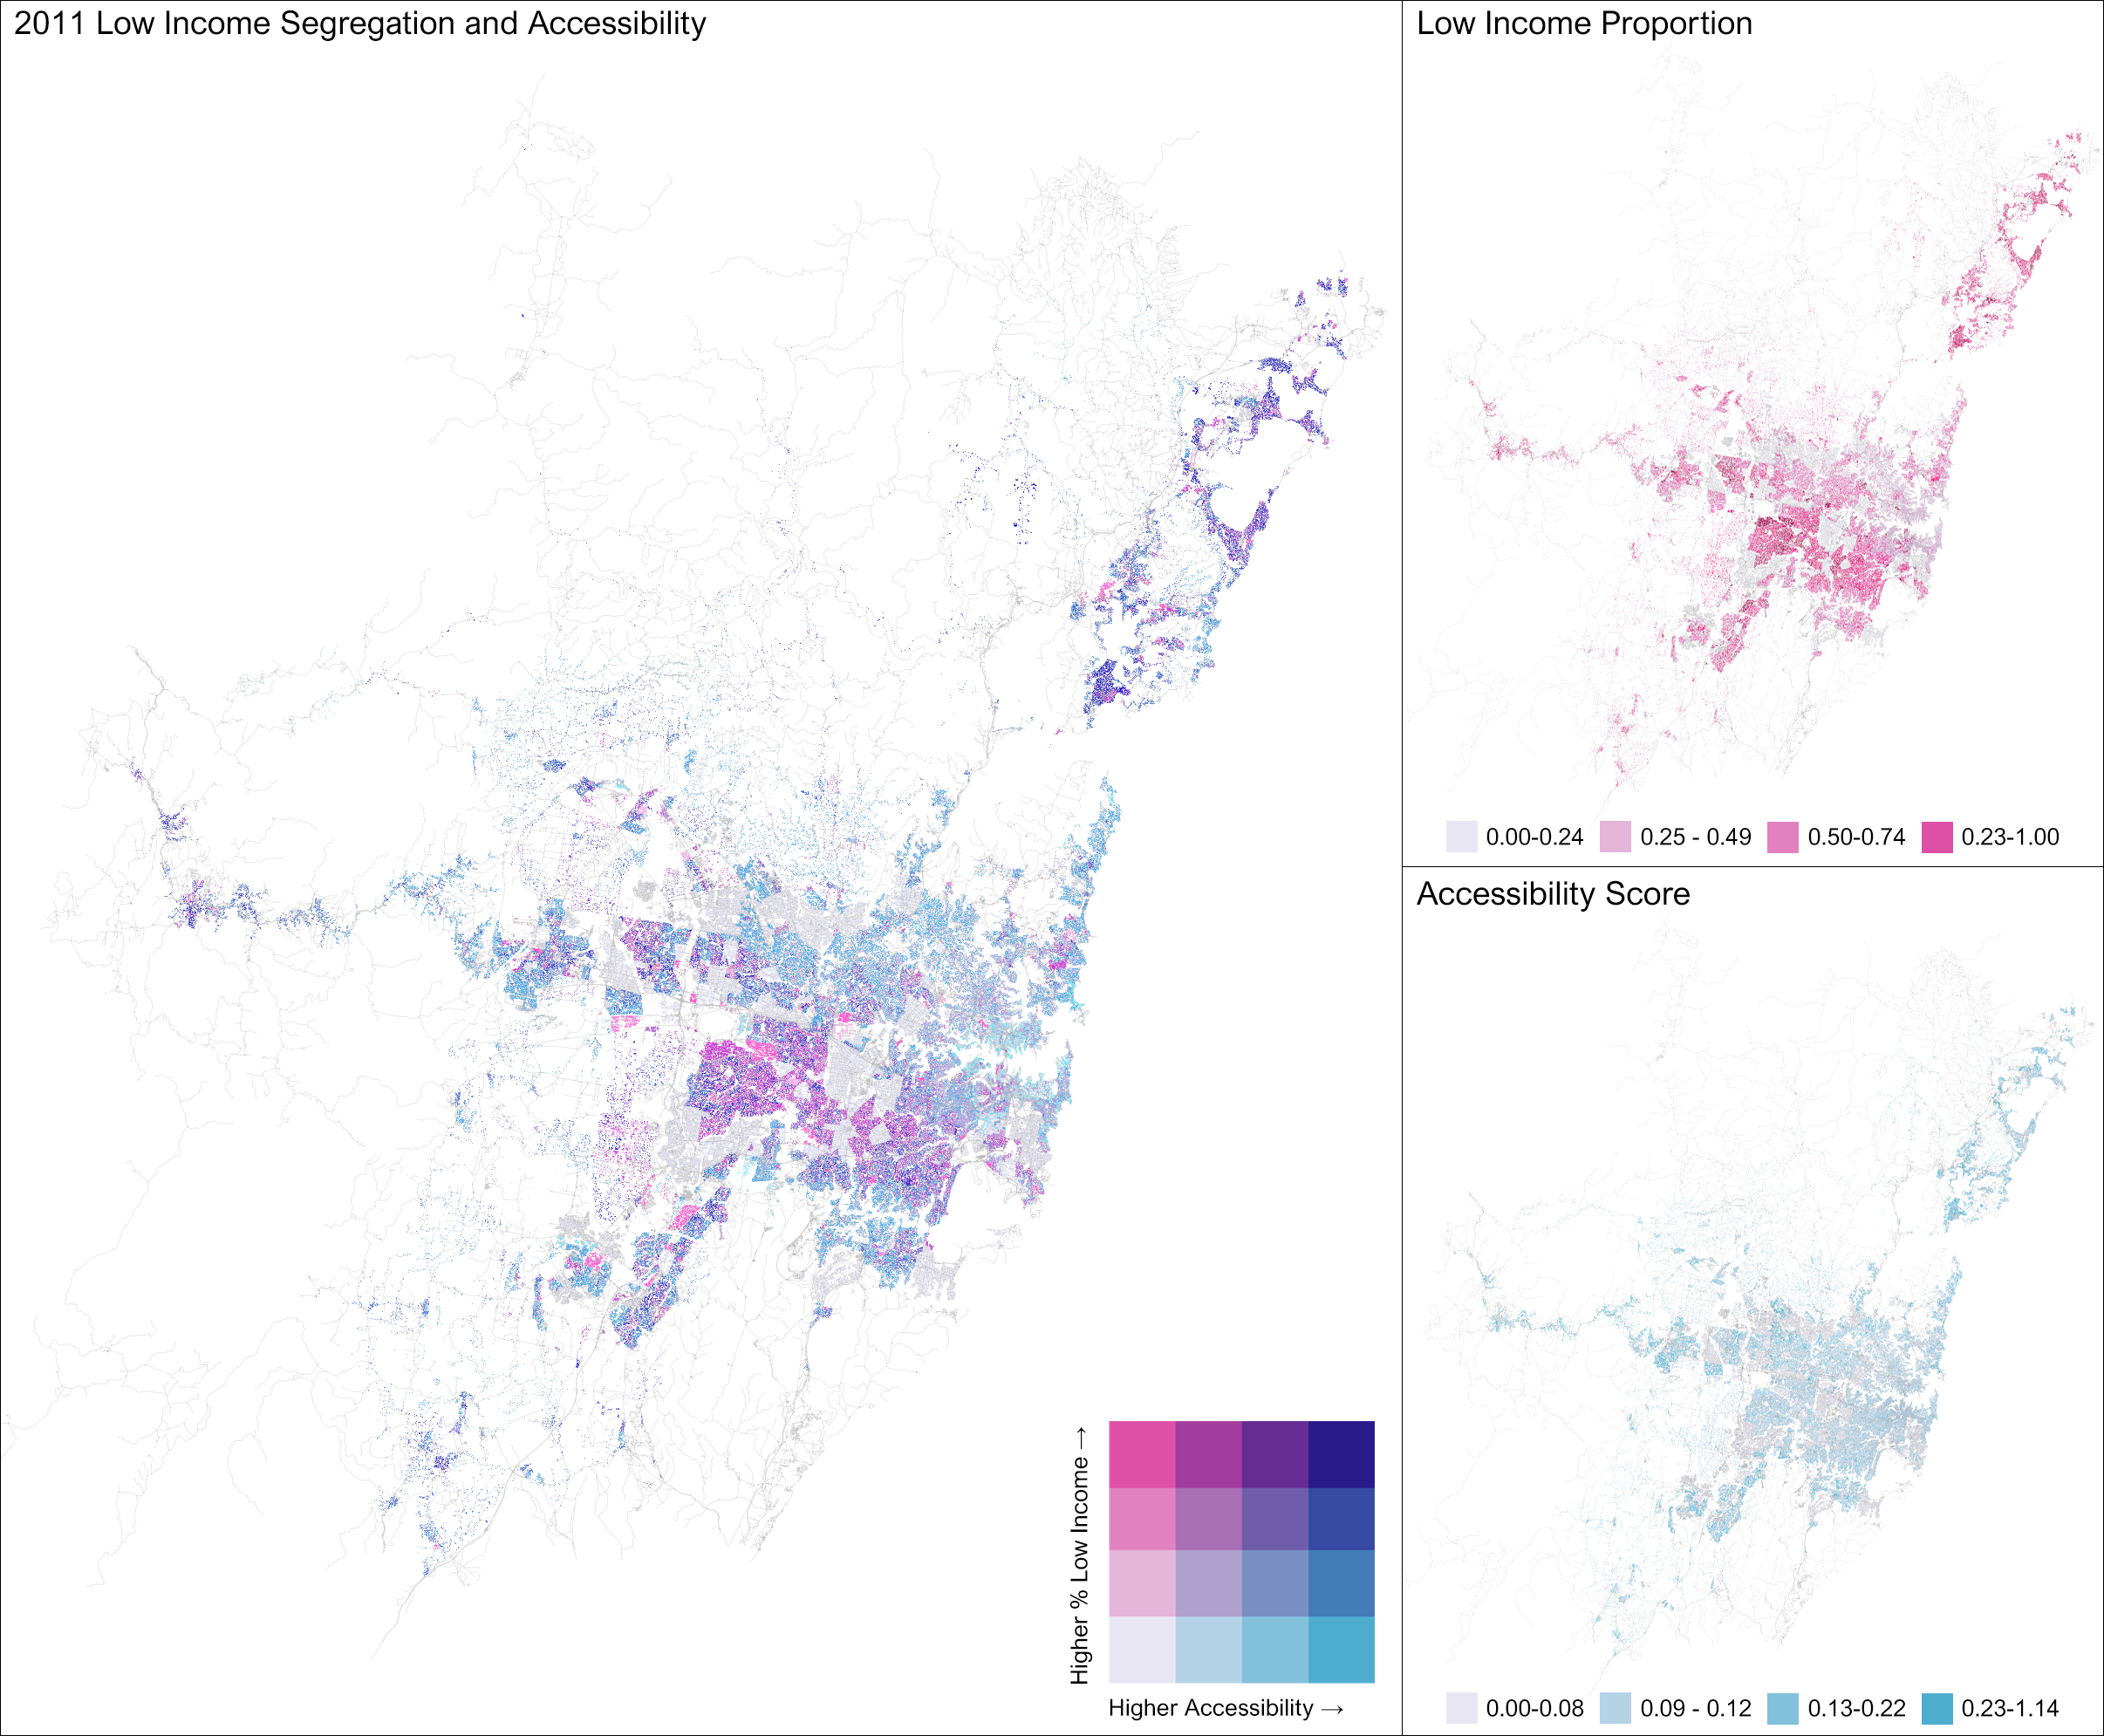
\includegraphics[width=\textwidth]{body/figures/low_inc_11.png}
    \caption{Bivariate Graphs: 2011 Accessibility and Income Segregation}
    \label{fig:my_label}
\end{sidewaysfigure}
}

\afterpage{
\begin{sidewaysfigure}[ht]
    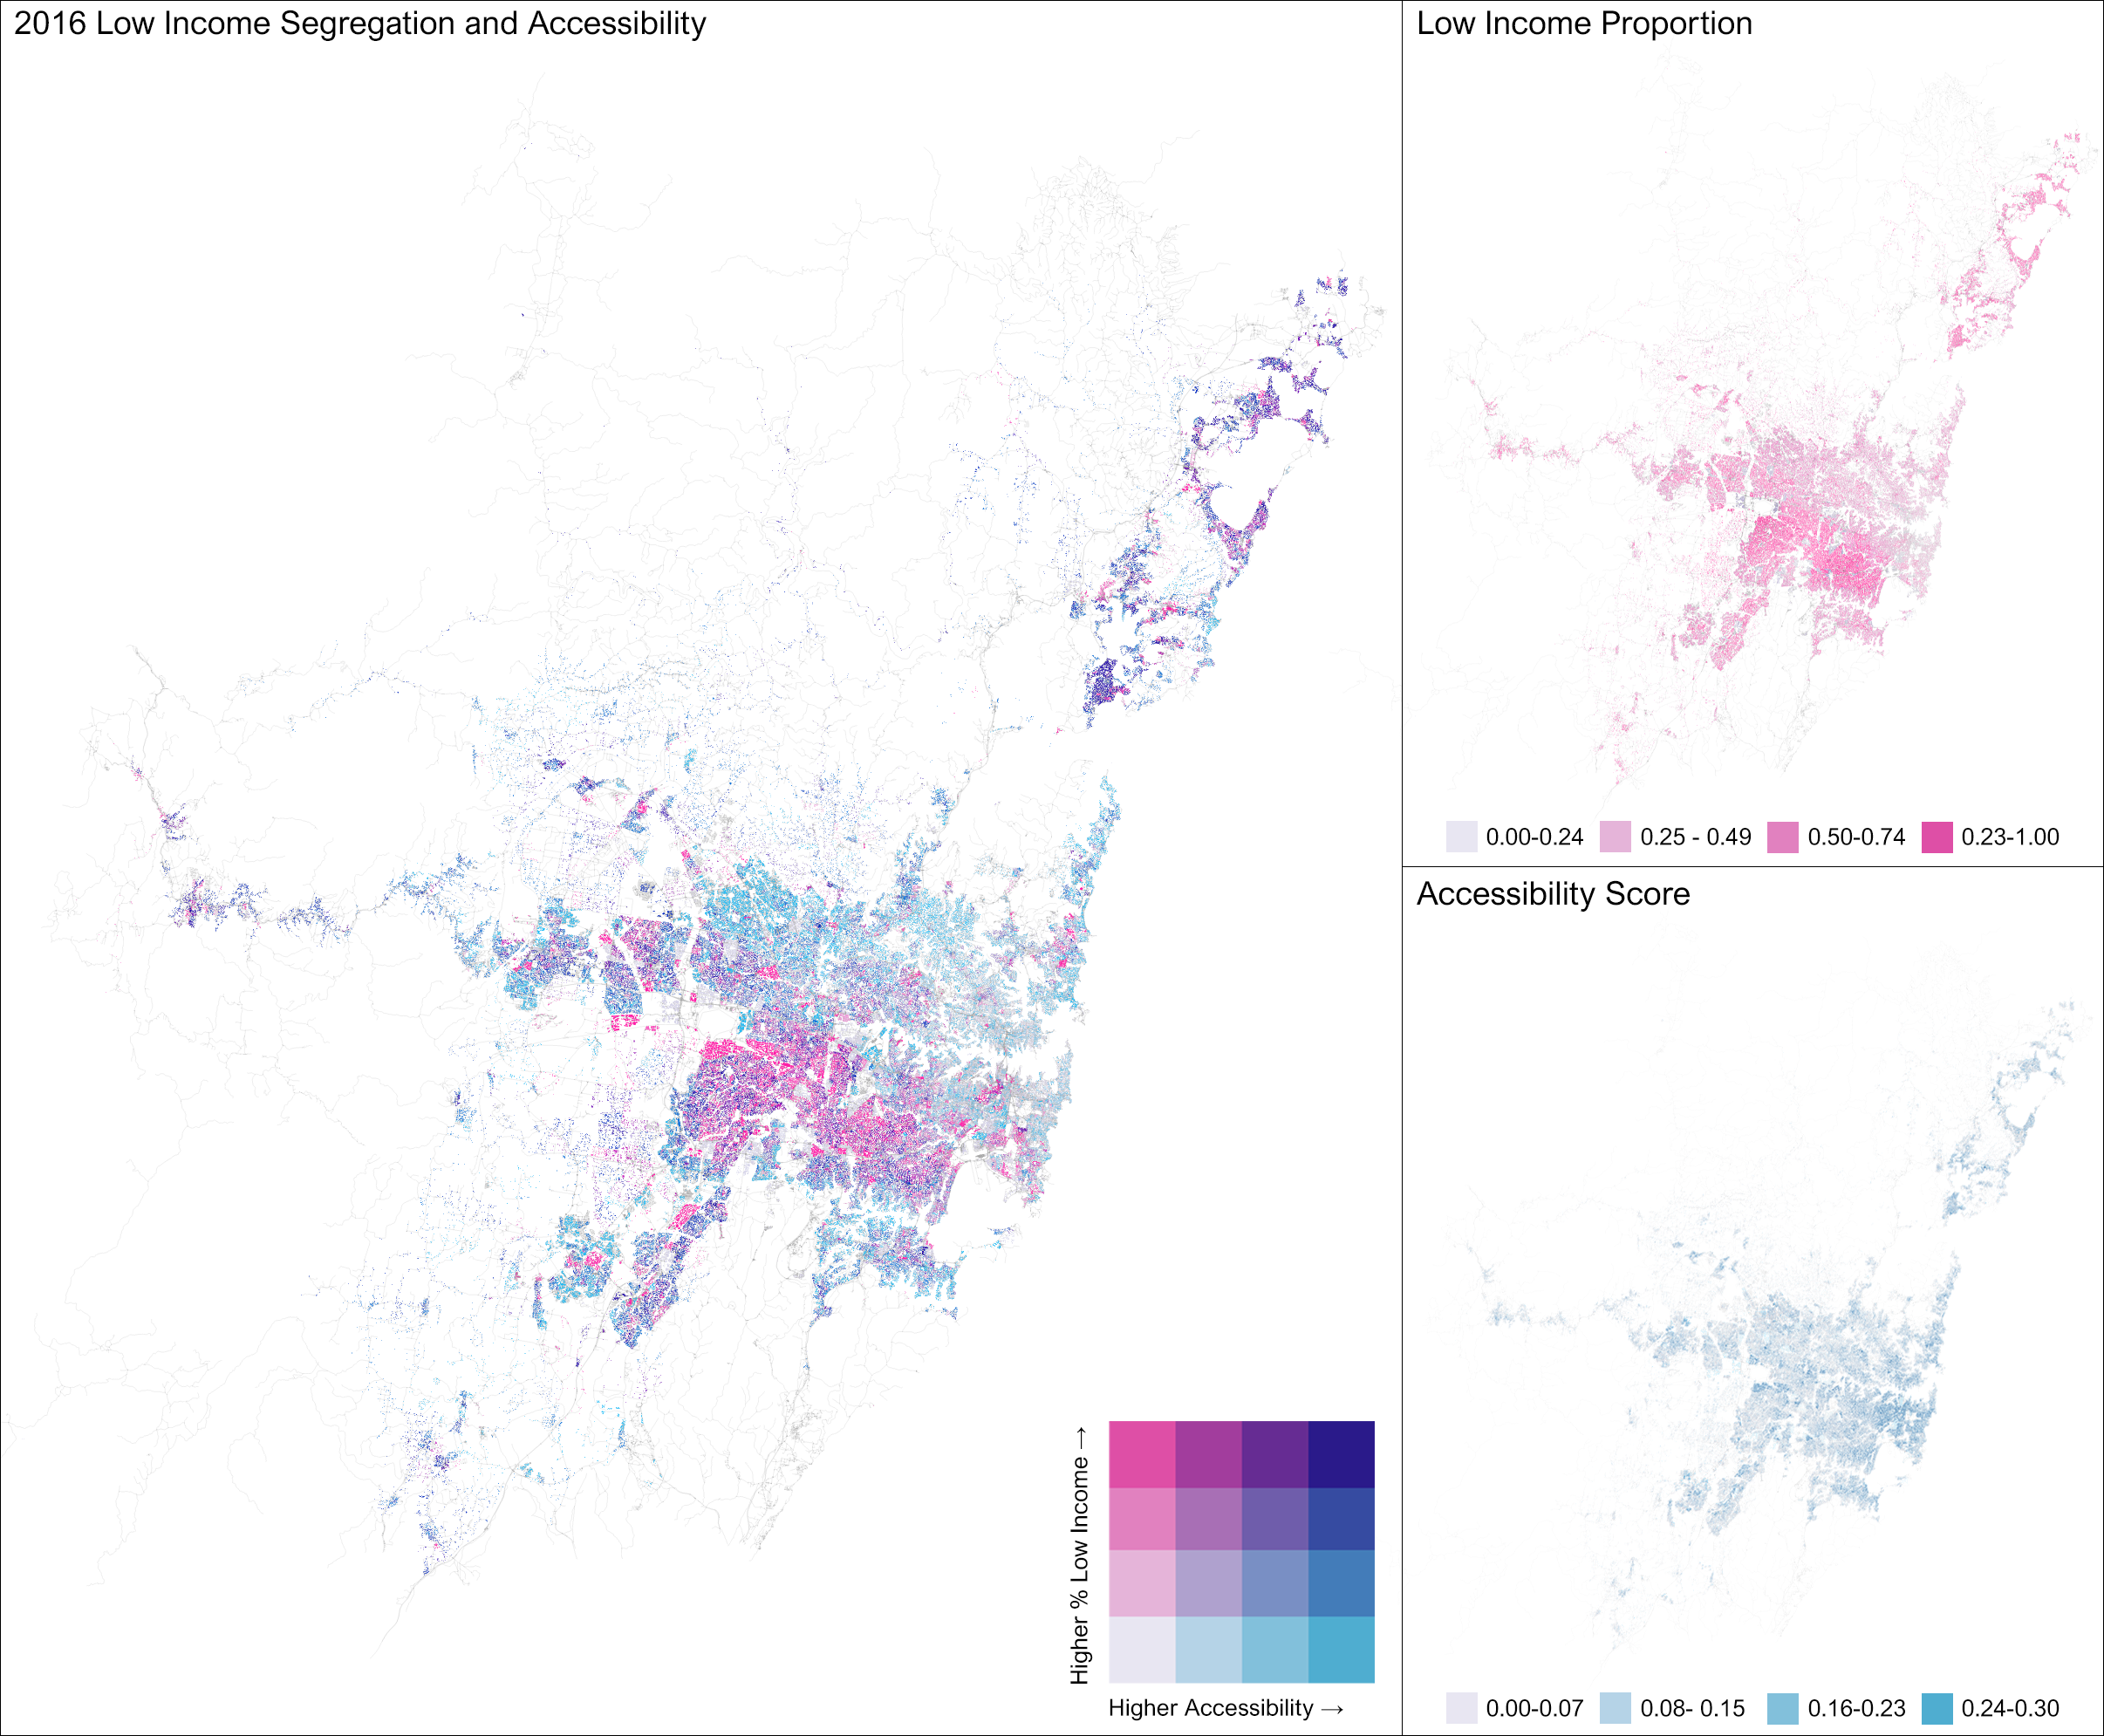
\includegraphics[width=\textwidth]{body/figures/low_inc_16.png}
    \caption{Bivariate Graphs: 2016 Accessibility and Income Segregation}
    \label{fig:my_label}
\end{sidewaysfigure}
}

\section{Discussion}

\section{Conclusion}
 